% Conditional UNIQUE: systems paper for ICDE (IEEEtran conference format).
% Status: restructured 2026-10-28 around soundness, coverage, cost and gains of the PostgreSQL
% prover; the axiomatisation, discovery theory and secondary experiments are in the appendix
% (extended version only). Evidence: experiments/sql_unique, experiments/tpcds.
\documentclass[conference]{IEEEtran}
\IEEEoverridecommandlockouts
\usepackage{amsmath,amssymb,amsthm}
\usepackage{booktabs}
\usepackage{array}
\usepackage{algorithm}
\usepackage{algpseudocode}
\usepackage{xcolor}
\usepackage{url}
\usepackage{balance}
\usepackage{tikz}
\usepackage{pgfplots}
\pgfplotsset{compat=1.18}
\usetikzlibrary{positioning,arrows.meta}
% Clickable URLs, cross-references and citations; URLs in dark blue, internal links in black.
\usepackage[colorlinks=true,urlcolor=blue!60!black,linkcolor=black,citecolor=black]{hyperref}
\hypersetup{pdftitle={When Can the Planner Trust a Filtered Unique Index?},pdfauthor={Ziheng Wei, Sebastian Link}}

\newtheorem{theorem}{Theorem}
\newtheorem{lemma}[theorem]{Lemma}
\newtheorem{proposition}[theorem]{Proposition}
\newtheorem{corollary}[theorem]{Corollary}
\theoremstyle{definition}
\newtheorem{definition}[theorem]{Definition}
\newtheorem{example}[theorem]{Example}

\newcommand{\todo}[1]{\textcolor{red}{[TODO: #1]}}
\newcommand{\sql}[1]{\texttt{#1}}
\newcommand{\nul}{\texttt{null}}
\newcommand{\NN}{\mathit{NN}}
\newcommand{\Sig}{\Sigma}
\newcommand{\U}[1]{\mathrm{U}(#1)}
\newcommand{\Ueq}[1]{\mathrm{U}^{=}(#1)}
\newcommand{\any}{\square}
\newcommand{\tpl}[1]{\ensuremath{\langle #1\rangle}}
\newcommand{\inn}[1]{{\in}#1}
\newcommand{\nin}[1]{{\notin}#1}
\newcommand{\scope}{\mathrm{sc}}
\newcommand{\prof}{\mathrm{prof}}
\newcommand{\Prof}{\mathrm{Prof}}
\newcommand{\consts}{\mathrm{consts}}
\newcommand{\ag}{\approx}
% The appendix is for the extended version; ICDE submissions allow no appendix.
% Set \extendedfalse for the submission.
\newif\ifextended
\extendedtrue


\begin{document}

\title{When Can the Planner Trust\\ a Filtered Unique Index?}

\author{\IEEEauthorblockN{Ziheng Wei}
\IEEEauthorblockA{School of Computer Science, Wuhan University\\
Wuhan, Hubei, China\\
\href{mailto:ziheng.wei@whu.edu.cn}{ziheng.wei@whu.edu.cn}\\
ORCID: \href{https://orcid.org/0000-0002-1859-0374}{0000-0002-1859-0374}}
\and
\IEEEauthorblockN{Sebastian Link}
\IEEEauthorblockA{School of Computer Science, The University of Auckland\\
Auckland, New Zealand\\
\href{mailto:s.link@auckland.ac.nz}{s.link@auckland.ac.nz}\\
ORCID: \href{https://orcid.org/0000-0002-1816-2863}{0000-0002-1816-2863}}}

\maketitle

\begin{abstract}
Applications often need a key that holds on part of a table only. An e-mail address must be unique among the
accounts that are not deleted, and a product code among the current versions. Applications declare such keys as
filtered (partial) unique indexes, which make up one in nine unique indexes in ten open-source application schemas.
Query optimisers could use these keys, as they use ordinary ones, to remove redundant joins and \sql{DISTINCT}s. In
practice they do not trust them. PostgreSQL did, returned wrong results, and has ignored them since 2023.
CockroachDB and SQL Server ignore them too, and SQLite only matches predicates word for word. We show when trust is sound. A proof of
uniqueness may use only the table's own restrictions, and it must use the \nul\ semantics of the rewrite it serves.
Rewrites shaped like joins need uniqueness with \nul s distinct, and rewrites shaped like groupings need it with \nul s
not distinct. Under two side conditions, the first question can be decided in polynomial time. The second is coNP-complete. Yet nearly
all implications between the indexes of real schemas are easy. Our prover combines all unique indexes and \sql{CHECK}
constraints of a table and carries uniqueness through joins. It fits into PostgreSQL~18.6 with 38 changed planner lines,
and into CockroachDB. It changed no result on 1{,}000{,}000 random queries. On catalogs over 226 real tables, it allows
exactly the rewrites that the catalogs imply, where stock PostgreSQL allows none. It adds 0.03\,ms to planning. Users' queries over
Stack Exchange run up to $3.3\times$ faster, mostly through keys carried through joins, and queries we wrote over
MusicBrainz run up to $4.9\times$ faster.
\end{abstract}

\begin{IEEEkeywords}
query optimisation, filtered unique indexes, partial indexes, keys, null markers, implication
\end{IEEEkeywords}

%=====================================================================
\section{Introduction}\label{sec:intro}
%=====================================================================

\paragraph*{Keys that hold on part of a table} Many business rules are keys with an exception. A user's
e-mail address must be unique among the accounts that are not deleted. A deleted account may keep its address,
and a new account may then reuse it. An item identifier must be unique among the current versions of a slowly
changing dimension, while old versions repeat it. A template name must be unique within one account, one inbox,
or the whole installation, depending on its scope. SQL's \sql{UNIQUE} constraint always holds on the whole table,
so it cannot state any of these rules. Database systems offer \emph{filtered unique indexes} instead. Such an
index enforces uniqueness only over the rows that satisfy its predicate:
\begin{center}
\sql{CREATE UNIQUE INDEX ON users (email) WHERE deleted\_at IS NULL;}
\end{center}
PostgreSQL and SQLite call them partial indexes~\cite{Sto89,PGDoc,SQLiteDoc}, and SQL Server calls them filtered
indexes~\cite{SQLServerDoc}. Frameworks such as Rails and Django generate them from model declarations. In ten
open-source application schemas we found 174 of them among 1{,}513 unique indexes, and seven of the
ten applications use them (Section~\ref{sec:practice}).

\paragraph*{What an optimiser does with keys} A unique index is an integrity rule, but it is also a fact that the
optimiser can use. Object-relational mappers, reporting tools and views often generate queries with work that a key
makes redundant. Optimisers remove this work with a family of \emph{uniqueness-based rewrites}~\cite{PL94,SSM96}:
\begin{itemize}
\item \emph{Left-join removal.} A view may left-join an optional table to show its columns. Suppose a query does not
  use these columns, and the joined table has at most one match for each outer row. Then the join changes nothing,
  and it can be dropped.
\item \emph{Semi-join to join.} A predicate \sql{x IN (SELECT y \ldots)} can be planned as an ordinary join only after
  duplicate values of \sql{y} are removed. A join gives the optimiser more freedom in the join order. If \sql{y} is a
  key, there are no duplicates to remove.
\item \emph{\sql{DISTINCT} and \sql{GROUP BY} removal.} If the selected or grouping columns contain a key, every row is
  already distinct, and every group has one row.
\item \emph{Inner-unique joins.} If each outer row has at most one partner, the join can stop searching after the first
  match. The cost model can also take this into account.
\end{itemize}
All four systems we study apply some of these rewrites with ordinary unique indexes. With filtered ones, the picture
is different (Section~\ref{sec:systems}):
\begin{itemize}
\item \emph{PostgreSQL} once used a partial unique index whenever the query's clauses implied its predicate. This
  led to wrong results (bug \#17975). Since June 2023, every supported version ignores partial indexes in all of
  these rewrites~\cite{PGBug17975}, even when the query's predicate \emph{is} the index's predicate. Users have asked
  for the rewrites back~\cite{Car19}. A patch proposed in 2026 addresses estimates only~\cite{Yan26}.
\item \emph{SQLite} removes a left join over a partial unique index only if the query's terms match the index predicate
  word for word. For example, the query term \sql{st = 0} does not match the index predicate \sql{st IN (0, 1)}. SQLite never removes \sql{DISTINCT}
  with a partial index.
\item \emph{CockroachDB} and \emph{SQL Server} use filtered unique indexes for none of these rewrites.
\end{itemize}

\paragraph*{Two pitfalls} The systems have good reason to be careful. A filtered key holds only on its scope. A
rewrite that relies on the key is sound only if every row that the rewrite reasons about lies in that scope. There
are two ways to get this wrong, and both have happened.

The first concerns \emph{which conditions may establish the scope}. Take the index \sql{UNIQUE (k) WHERE c IS NOT
NULL} on a table \sql{t}, and the query \sql{o JOIN t ON o.k = t.k JOIN u ON t.c = u.c}. The second join keeps only
the rows of \sql{t} whose \sql{c} is not \nul. So it seems that \sql{t} is unique on \sql{k}. But the first join is
evaluated before the second, on all rows of \sql{t}. If the planner marks the first join as unique, it stops at the
first match on \sql{k}. That match may have \nul\ in \sql{c}, and the second join then discards it. The row that would
have survived is never found. This is PostgreSQL's bug \#17975. The lesson is that a uniqueness proof must hold for
the rows of a table \emph{before} any join. It may therefore use only the table's own restrictions.

The second pitfall concerns \emph{\nul}. By default, a SQL unique index allows any number of rows with \nul\ in the
key, because \nul\ does not equal \nul. A join on the key never matches \nul. Such an index therefore still proves that a
join finds at most one partner. But \sql{DISTINCT} and \sql{GROUP BY} put all \nul s into one group. The same index
therefore does not prove that \sql{DISTINCT} is redundant: two rows with a \nul\ key form one group, not two.

Both pitfalls have measurable effects. On random schemas, a planner that proves an index's predicate from another join's
clause, as PostgreSQL did, changes 442 of 20{,}000 query results. On 217 open-data tables, a planner that ignores the
\nul\ semantics would remove 22{,}171 \sql{DISTINCT}s, and 3{,}121 of these removals, on 133 of the tables, would be
wrong (Section~\ref{sec:experiments}).

\begin{figure}[t]
\centering\footnotesize
\begin{tabular}{@{}rll@{}}
\multicolumn{3}{@{}l}{\sql{users}}\\\toprule
\sql{id} & \sql{email} & \sql{deleted\_at}\\\midrule
1 & \sql{a@x} & \nul\\
2 & \sql{a@x} & 2024-03-01\\
3 & \sql{b@x} & \nul\\\bottomrule
\end{tabular}\hfill
\begin{tabular}{@{}rll@{}}
\multicolumn{3}{@{}l}{\sql{user\_emails}}\\\toprule
\sql{user\_id} & \sql{address} & \sql{is\_primary}\\\midrule
1 & \sql{a@x} & true\\
1 & \sql{a2@y} & false\\
3 & \sql{b@x} & true\\\bottomrule
\end{tabular}

\smallskip
\begin{tabular}{@{}l@{}}
\sql{UNIQUE (email) WHERE deleted\_at IS NULL}\\
\quad $\{\tpl{\mathit{deleted\_at}{:}\,\bot}\}:\U{\mathit{email}}$, \sql{email} \sql{NOT NULL}\\
\sql{UNIQUE (user\_id, is\_primary) WHERE is\_primary}\\
\quad $\{\tpl{\mathit{is\_primary}{:}\,\mathit{true}}\}:\U{\mathit{user\_id},\mathit{is\_primary}}$\\[3pt]
\sql{SELECT DISTINCT u.email, e.address FROM users u}\\
\sql{\ \ JOIN user\_emails e ON e.user\_id = u.id}\\
\sql{\ \ \ \ AND e.is\_primary}\\
\sql{\ \ WHERE u.deleted\_at IS NULL}
\end{tabular}

\smallskip
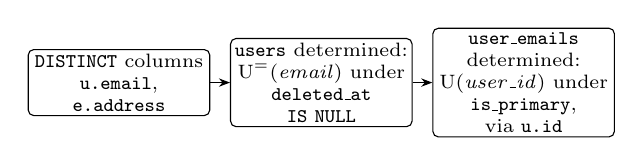
\begin{tikzpicture}[node distance=2.5mm, every node/.style={draw, rounded corners=2pt,
    align=center, inner sep=1.5pt, font=\scriptsize, text width=2.2cm}, >={Stealth[length=4pt]}]
\node (g) {\sql{DISTINCT} columns\\\sql{u.email}, \sql{e.address}};
\node (u) [right=of g] {\sql{users} determined:\\$\Ueq{\mathit{email}}$ under\\\sql{deleted\_at IS NULL}};
\node (e) [right=of u] {\sql{user\_emails} determined:\\$\U{\mathit{user\_id}}$ under\\\sql{is\_primary}, via \sql{u.id}};
\draw[->] (g) -- (u); \draw[->] (u) -- (e);
\end{tikzpicture}
\caption{Running example. Each live user has one e-mail address, and each user has one primary address. Hence every
row of the join is determined by its \sql{DISTINCT} values, and \sql{DISTINCT} is redundant. Without \sql{e.is\_primary},
user~1 has two rows. Without \sql{deleted\_at IS NULL}, users 1 and 2 share \sql{a@x}. If \sql{email} were nullable,
$\U{\mathit{email}}$ would not give $\Ueq{\mathit{email}}$, because \sql{DISTINCT} puts all \nul s into one group.}
\label{fig:example}
\end{figure}

\paragraph*{Our approach} We read a filtered unique index as a constraint, which we call a \emph{conditional
\sql{UNIQUE}}. The planner's question then becomes one of \emph{implication} between constraints. Consider the unique
indexes of a table, together with its \sql{NOT NULL} columns and \sql{CHECK} constraints. Do they guarantee, for every
possible content of the table, that the rows matching the query's restriction are unique on the columns that the
query joins or groups on? Implication concerns the declared constraints, not the current data, so its answer stays
correct when the data changes.

Implication also does more than match the query against one index at a time. Several indexes can together guarantee
a key that none of them states alone. A query's scope can differ from an index's scope and still lie within it. A
\sql{CHECK} constraint can exclude the rows that an index does not cover. Fig.~\ref{fig:example} shows a query whose
\sql{DISTINCT} is redundant only because two filtered keys are combined across a join.

If we ask the question with the table's own restrictions only, we avoid the first pitfall. If we ask it with the
\nul\ semantics that the rewrite needs, we avoid the second. The two semantics also differ in complexity. For
join-shaped rewrites, implication can be decided in polynomial time when the predicates are conjunctive and have no
inequalities or \sql{IN}-lists on the compared columns. For group-shaped rewrites, implication is coNP-complete. Under
the same conditions, it is hard only through nullable grouping columns that the query leaves open. Real schemas fall
on the easy side. Among the indexes of the ten applications, 2{,}953 of 2{,}960 implications are as easy as in the
first case. When an implication fails, a table of two rows shows why.

\paragraph*{What we found} We built a prover based on this theory into the planner of PostgreSQL~18.6, with 1{,}683
new lines of C and 38 changed lines, and we ported it to CockroachDB.
\begin{itemize}
\item \emph{It is sound.} On 1{,}000{,}000 random queries it changed 154{,}532 plans and no result. If any of its
  safeguards is removed, the random queries or a feature test detect the error.
\item \emph{It is exact on real catalogs.} We declared catalogs of filtered unique indexes over 226 real tables. The
  prover allows exactly the rewrites that each catalog implies, which is more than one index at a time allows. Stock
  PostgreSQL allows none.
\item \emph{It is cheap.} It adds 0.03\,ms to planning in the median.
\item \emph{Its gains depend on who writes the queries.} Application code, transformation code and reports use filtered
  keys for integrity, and they rarely filter on the keys' scopes. Users who query Stack Exchange do. Their queries
  gain up to $3.3\times$, but mostly through ordinary keys carried through joins, which the prover adds to PostgreSQL.
  Views over versioned data lose every join they add. Queries we wrote over MusicBrainz gain up to $4.9\times$.
\end{itemize}

\paragraph*{Contributions}
\begin{enumerate}
\item \emph{The state of practice.} We study filtered unique indexes in ten application schemas, and what
  PostgreSQL, SQLite, CockroachDB and SQL Server do with them (Section~\ref{sec:practice}).
\item \emph{The complexity of the planner's question.} For conditional \sql{UNIQUE} constraints under both \nul\
  semantics, implication is polynomial for join-shaped rewrites under two side conditions. It is coNP-complete for
  group-shaped rewrites, but fixed-parameter tractable under the same conditions. It is coNP-complete whenever a side
  condition fails (Sections~\ref{sec:model} and~\ref{sec:reasoning}). A finite axiomatisation is in \ifextended the
  appendix\else the extended version\fi.
\item \emph{A sound prover} in PostgreSQL~18.6. It is exact for one relation over the indexes it translates. It serves
  the existing join rewrites and the reduction of \sql{GROUP BY}, adds the removal of \sql{DISTINCT}, reads \sql{CHECK}
  constraints, and carries both semantics through inner, left, semi- and anti-joins. We also port it to CockroachDB
  (Section~\ref{sec:planner}).
\item \emph{Evidence} of soundness, of exactness against four systems on real catalogs, of cost, and of gains on
  workloads grouped by who writes the queries (Section~\ref{sec:experiments}).
\end{enumerate}
\ifextended The appendix \else The extended version~\cite{EXT} \fi contains the proofs, the axiomatisation, a
recommender for filtered unique indexes, and further experiments.


%=====================================================================
\section{Filtered Unique Indexes in Practice}\label{sec:practice}
%=====================================================================

\subsection{In application schemas}\label{sec:schemas}

We took the schemas of ten open-source applications that use PostgreSQL: GitLab, Mastodon, Forem, Chatwoot,
Loomio, Consul, Open Food Network, Maybe, DocuSeal and Campsite. For GitLab we read its \sql{structure.sql}, and for
the others their Rails \sql{schema.rb}. We parsed their unique indexes, primary keys, \sql{UNIQUE} constraints and
\sql{NOT NULL} columns. GitLab keeps a copy of some indexes for each partition, and we count these copies once.
Table~\ref{tab:schemas} summarises the schemas.

\begin{table}[t]
\caption{Unique indexes in ten application schemas}\label{tab:schemas}
\centering\small
\setlength{\tabcolsep}{4pt}
\begin{tabular}{lrrrr}
\toprule
Application & Tables & Unique & Filtered & $\ge2$ per table \\
\midrule
GitLab & 1{,}135 & 930 & 128 & 26 \\
Mastodon & 122 & 91 & 14 & 3 \\
Forem & 131 & 110 & 12 & 4 \\
Chatwoot & 109 & 93 & 9 & 2 \\
Loomio & 76 & 68 & 5 & 1 \\
DocuSeal & 44 & 36 & 3 & 0 \\
Maybe & 59 & 30 & 3 & 1 \\
Three others$^{*}$ & 323 & 155 & 0 & 0 \\
\midrule
Total & 1{,}999 & 1{,}513 & 174 & 37 \\
\bottomrule
\end{tabular}

\smallskip\footnotesize $^{*}$Campsite, Consul, Open Food Network
\end{table}

The predicates fall into a few shapes:
\begin{itemize}
\item \emph{Excluding \nul\ keys} (87), as in \sql{UNIQUE (k) WHERE k IS NOT NULL}. All 14 of Mastodon's filtered
  indexes and 63 of GitLab's have this shape. Under \sql{NULLS DISTINCT} the predicate changes nothing, so such an
  index states an ordinary key. The predicate only keeps the index small, or it is a habit from SQL Server, where it is
  the only way to allow several \nul s.
\item \emph{A constant or flag} (33): \sql{status = 0}, \sql{published IS TRUE}, \sql{rule\_type = 2}.
\item \emph{A missing value in another column} (26): \sql{ended\_at IS NULL}, \sql{resolved\_at IS NULL}. These express
  soft deletion, current versions and open episodes.
\item \emph{IN-lists} (9): \sql{status = ANY (ARRAY[0, 1])}.
\item \emph{Conjunctions of the above} (5). For example, Chatwoot has three scopes for e-mail templates: one per
  installation (\sql{account\_id IS NULL AND inbox\_id IS NULL}), one per account (\sql{account\_id IS NOT NULL AND
  inbox\_id IS NULL}), and one per inbox.
\item \emph{Inequalities} (14): \sql{package\_type = 7 AND status <> 4}, \sql{custom\_domain <> ''}.
\end{itemize}
Six indexes have keys that are expressions, such as \sql{lower(email)}. The other 168 have predicates built from
\sql{=}, \sql{<>}, \sql{IN}, \sql{IS [NOT] NULL}, \sql{AND} and \sql{OR}. In the terms of Section~\ref{sec:model}, all
168 are conditions with one template: 159 are conjunctions, and 9 are \sql{IN}-lists. SQL writes an \sql{IN}-list as a
disjunction, but one template entry can hold it. In the 37 tables with two or more filtered unique indexes, a planner that
looks at one index at a time can miss what the indexes say together. Only two filtered indexes are
implied by others, in both cases by the primary key. Developers thus do not declare filtered indexes redundantly.
\ifextended
Beyond these applications, we looked at the SQL files of SchemaPile~\cite{SchemaPile}, which holds 22{,}989
permissively licensed schemas from GitHub. There, filtered indexes make up 12.9\% of the \sql{CREATE UNIQUE INDEX}
statements in SQL Server files (118 of 913) and 5.4\% in PostgreSQL files (182 of 3{,}362). Their predicates have the
same shapes: constants and flags, \nul\ tests on other columns, and the exclusion of \nul\ keys. Of the 356 filtered
unique indexes in all dialects, 69 use conjunctions, only 8 use \sql{OR}, and 6 use range comparisons.

\paragraph*{In analytics code} Data warehouses built with dbt state keys as tests. In the two largest public dbt
projects we found, 38 of 369 uniqueness tests have a scope (\sql{where:}). In 27 of them, the scope expresses a
documented exception to the key.

\paragraph*{In open data} MusicBrainz publishes its PostgreSQL schema and data, with 17 filtered unique indexes. On
13 alias tables, \sql{(entity, locale) WHERE primary\_for\_locale AND locale IS NOT NULL} allows at most one primary
alias per entity and locale. Artists and labels are unique by name, and a comment tells namesakes apart: \sql{(name) WHERE comment IS
NULL} and \sql{(name, comment) WHERE comment IS NOT NULL}. This pair is the encoding of $\Ueq{}$ in
Proposition~\ref{prop:translate}. Since \sql{comment} became \sql{NOT NULL}, the second index states an ordinary key,
which PostgreSQL ignores because the index is partial. Every key holds in the data of 28 October 2026.

\else
The same shapes occur beyond these applications. In SchemaPile~\cite{SchemaPile}, a corpus of 22{,}989 schemas from
GitHub, filtered indexes make up 12.9\% of the unique indexes in SQL Server files and 5.4\% in PostgreSQL files. In the
two largest public dbt projects, 38 of 369 uniqueness tests have a scope. MusicBrainz, whose schema and data are
public, declares 17 filtered unique indexes, and all of them hold in its data. Among them are \sql{(name) WHERE comment
IS NULL} and \sql{(name, comment) WHERE comment IS NOT NULL}, the encoding of $\Ueq{}$ in
Proposition~\ref{prop:translate}.

\fi
\subsection{In optimisers}\label{sec:systems}

Table~\ref{tab:systems} lists the uniqueness-based optimisations of PostgreSQL~18.6, SQLite~3.54, CockroachDB~26.3
and SQL Server~2025. For each, it shows whether a filtered unique index enables it. We tested each system with an
ordinary unique index on $k$ and a partial unique index on $k$ \sql{WHERE d IS NULL}, using queries with exactly that
predicate. We then traced each behaviour to the source code.

\begin{table}[t]
\caption{Uniqueness-based optimisations with a plain and a filtered unique
index whose predicate equals the query predicate}\label{tab:systems}
\centering\small\setlength{\tabcolsep}{4pt}
\begin{tabular}{@{}llcc@{}}
\toprule
System & Optimisation & plain & filtered \\
\midrule
PostgreSQL 18 & left-join removal & yes & no \\
 & semi-join to join & yes & no \\
 & inner-unique join & yes & no \\
 & \sql{GROUP BY} column removal & yes & no \\
 & self-join elimination & yes & no \\
 & \sql{DISTINCT} removal & no & no \\
\midrule
SQLite 3.54 & \sql{DISTINCT} removal & yes & no \\
 & left-join omission & yes & syntactic \\
\midrule
CockroachDB & left-join removal & yes & no \\
 & \sql{DISTINCT} removal & yes & no \\
 & \sql{GROUP BY} reduction & yes & no \\
\midrule
SQL Server & left-join removal & yes & no \\
 & semi-join to join & yes & no \\
 & \sql{DISTINCT} removal & yes & no \\
 & \sql{GROUP BY} removal & yes & no \\
\bottomrule
\end{tabular}
\end{table}

\ifextended
\paragraph*{PostgreSQL} Before planning, \sql{check\_index\_predicates} sets the \sql{predOK} flag of a partial index
if \sql{predicate\_implied\_by} proves the index's predicate from the relation's restrictions. Until 2023,
\sql{relation\_has\_unique\_index\_for} accepted partial indexes with \sql{predOK} set. This function is the uniqueness
test behind left-join removal, semi-join reduction and inner-unique joins. But \sql{predOK} may be proved from join
clauses that are evaluated only after the inner relation is read. The planner could therefore treat a relation as unique
when it is not. The fix (commit \sql{7fcd7ef2a9}, back-patched to all supported versions) excludes every index with a
predicate from \sql{relation\_has\_unique\_index\_for} and \sql{rel\_supports\_distinctness}. Version~18 added the reduction
of \sql{GROUP BY} by unique indexes and the elimination of self-joins, and both skip partial indexes from the start.
Partial indexes with \sql{predOK} now matter only for the estimated number of distinct values. PostgreSQL removes
\sql{DISTINCT} for no base table, filtered or not.

\paragraph*{SQLite} The function \sql{isDistinctRedundant} skips partial indexes. Left-join omission relies on a flag
that marks the access path of the inner table as returning at most one row. A partial unique index sets this flag when
\sql{whereUsablePartialIndex} finds, for each conjunct of the predicate, a term of the \sql{ON} or \sql{WHERE} clause on
that table that implies it. The test, \sql{sqlite3ExprImpliesExpr}, accepts the same expression, one branch of an
\sql{OR}, or \sql{IS NOT NULL} after a comparison that rejects \nul. This is sound but fragile. Both \sql{b.st = 0}
against \sql{WHERE st IN (0, 1)} and \sql{NOT (b.d IS NOT NULL)} against \sql{WHERE d IS NULL} keep the join, and two
indexes are never combined.

\paragraph*{CockroachDB} The optimiser derives a table's keys in \sql{MakeTableFuncDep}. This function skips partial
unique indexes and partial \sql{UNIQUE WITHOUT INDEX} constraints, because their keys hold on part of the table only. It
does add such a key to a scan \emph{of} the partial index. But that scan is an alternative found during exploration,
while join elimination, \sql{DISTINCT} removal and grouping reduction are normalisation rules applied to the table's
canonical scan. None of these rules used a partial key in our tests. For example, \sql{DISTINCT k} stays above a scan of
the partial unique index on \sql{k}, even for \sql{UNIQUE (k) WHERE k IS NOT NULL}.

\paragraph*{SQL Server} Filtered unique indexes have conjunctive predicates of comparisons and \sql{IN}-lists, and their
\sql{UNIQUE} treats \nul\ as a value~\cite{SQLServerDoc}. Range comparisons are outside our language, so an index that
uses one cannot serve as a premise. White~\cite{White13} shows that the optimiser costs a one-to-one join over filtered
unique indexes as many-to-many, and he recommends redundant predicates or indexed views as workarounds. We tested SQL
Server~2025 (RTM-CU10, Developer edition) in the same way as the other systems. With a unique constraint, it removes the
left join and \sql{DISTINCT}, reduces \sql{GROUP BY}, and turns the semi-join into a join. With a filtered unique index on
the query's own predicate, it does none of these. It even keeps the aggregate for \sql{DISTINCT k} when it reads the
filtered index \sql{UNIQUE (k) WHERE k IS NOT NULL}.

\else
\paragraph*{Why each system declines} \emph{PostgreSQL} proves a partial index's predicate from the query's clauses,
including join clauses that are evaluated only after the table is read. Until 2023, its uniqueness test accepted such
indexes, and this caused bug \#17975. The fix excludes every index with a predicate from all uniqueness-based rewrites.
A partial index now affects only the estimated number of distinct values. PostgreSQL removes \sql{DISTINCT} for no base
table. \emph{SQLite} marks the inner table of a left join as returning at most one row if, for every conjunct of the
index predicate, one term of the query implies it word for word. It accepts the same expression, one branch of an
\sql{OR}, or \sql{IS NOT NULL} after a comparison. This is sound but fragile, and it never combines two indexes.
\emph{CockroachDB} derives a table's keys from its unique indexes but skips partial ones, because their keys hold on part
of the table only. Its rules for join elimination, \sql{DISTINCT} removal and grouping reduction therefore never see
them. \emph{SQL Server}'s filtered unique indexes treat \nul\ as a value~\cite{SQLServerDoc}. Its optimiser costs a
one-to-one join over them as many-to-many~\cite{White13}. In our tests of SQL Server~2025, it used them for none of the
rewrites, not even for \sql{DISTINCT k} over a scan of \sql{UNIQUE (k) WHERE k IS NOT NULL}.


\fi
%=====================================================================
\section{Conditional UNIQUE}\label{sec:model}
%=====================================================================

A table schema is a finite set $R$ of columns, with a subset $\NN\subseteq R$ of columns declared \sql{NOT NULL}. A
\emph{table} over $R$ is a finite multiset of records. A record maps each column to a value or to \nul, and it has no
\nul\ on a column of $\NN$. As in SQL, a table may contain duplicate records.

\paragraph*{Predicates as templates} We bring index predicates and query restrictions into one normal form, so that
we can reason about both alike. A \emph{template} $\tau$ maps each column to an entry. The entries are $\any$
(anything), $\top$ (\sql{IS NOT NULL}), $\bot$ (\sql{IS NULL}), ${\in}S$ (\sql{= c} or \sql{IN (S)}), and ${\notin}S$
(\sql{<> c} or \sql{NOT IN (S)}), for a finite non-empty set $S$ of constants. A \nul\ matches only $\any$ and $\bot$,
because a comparison with \nul\ is never true in a \sql{WHERE} clause. A value $v$ matches $\any$ and $\top$. It matches
${\in}S$ if $v\in S$, and ${\notin}S$ if $v\notin S$. A record \emph{matches} $\tau$ if it matches every entry. A
\emph{condition} is a finite set of templates, and a record matches it if the record matches one of them. Every
predicate built from \sql{=}, \sql{<>}, \sql{IN}, \sql{NOT IN}, \sql{IS [NOT] NULL}, \sql{AND} and \sql{OR} over columns
and constants is a condition. To see this, bring the predicate into disjunctive normal form. Two entries on the same
column combine into one entry, or into a contradiction. A conjunctive predicate is a condition with one template. Range
comparisons are outside the language. We write $\tpl{d{:}\,\bot}$ for the template with $\bot$ on $d$ and $\any$
elsewhere.

\begin{definition}
A \emph{conditional} \sql{UNIQUE} \emph{constraint} has the form $C:\U{K}$ or $C:\Ueq{K}$ for a
condition $C$ and a set $K\subseteq R$. A table $r$ satisfies it if no two records of $r$, at different positions,
both match $C$ and agree on $K$. For $\U{K}$ (\sql{NULLS DISTINCT}), two records agree on $K$ if they have the same value
on every column of $K$. For $\Ueq{K}$ (\sql{NULLS NOT DISTINCT}), \nul\ also counts as equal to \nul.
\end{definition}

The filtered unique index of the introduction is $\{\tpl{\mathit{deleted\_at}{:}\,\bot}\}:\U{\mathit{email}}$. In
PostgreSQL and SQLite, \sql{CREATE UNIQUE INDEX \ldots\ WHERE P} states $C_P:\U{K}$. PostgreSQL's \sql{NULLS NOT DISTINCT}
variant and SQL Server's filtered unique index state $C_P:\Ueq{K}$. A primary key is $\{\tpl{}\}:\U{K}$ with
$K\subseteq\NN$. A key over no columns, $C:\U{\emptyset}$, says that at most one record matches $C$. PostgreSQL can state
it as a unique index on a constant expression.

\begin{lemma}[Pairs]\label{lem:pairs}
A set $\Sig$ of conditional \sql{UNIQUE} constraints implies $\varphi$ iff every table of at most
two records that satisfies $\Sig$ satisfies $\varphi$.
\end{lemma}

\begin{proof}
Violations are witnessed by two records, and every constraint holds on a sub-table of a table
that satisfies it.
\end{proof}

\paragraph*{Between the dialects} Each \nul\ semantics can be expressed by the other, which matters when a schema
moves between systems. For a nullable key column, $\U{}$ is $\Ueq{}$ restricted to the records without \nul\ on $K$. SQL
Server users write this as \sql{WHERE k IS NOT NULL}. In the other direction, SQLite and PostgreSQL before version~15
can express $\Ueq{}$ only with one index for each pattern of \nul s on the key:

\begin{proposition}[Translation]\label{prop:translate}
Let $F$ be the nullable columns of $K$. Then
\begin{align*}
C:\U{K}&\equiv C\wedge\tpl{F{:}\,\top}:\Ueq{K},\\
C:\Ueq{K}&\equiv\{\,C\wedge p_N:\U{K\setminus N}\;:\;N\subseteq F\,\},
\end{align*}
where $p_N$ has $\bot$ on $N$ and $\top$ on $F\setminus N$, and $C\wedge p$ refines every template
of $C$ by $p$ (dropping contradictory ones). The second equivalence uses $2^{|F|}$ constraints,
one per pattern of \nul s on the nullable key columns.
\end{proposition}

\ifextended
\begin{proof}
By Lemma~\ref{lem:pairs}, it suffices to compare which pairs of records the two sides forbid. Consider the first
equivalence. A pair that matches $C$ and agrees on $K$ with values has no \nul\ on $K$. So it matches
$C\wedge\tpl{F{:}\,\top}$, and it agrees on $K$ with \nul\ equal to \nul. Conversely, a pair that matches
$C\wedge\tpl{F{:}\,\top}$ has no \nul\ on $F$, and none on $K\setminus F\subseteq\NN$. For such a pair, agreeing on $K$
with \nul\ equal to \nul\ is the same as agreeing with values. Now consider the second equivalence. Suppose two records
match $C$ and agree on $K$ with \nul\ equal to \nul. On each column of $K$, they are both \nul\ or carry the same value.
So they have the same set $N\subseteq F$ of \nul\ columns on $K$, they both match $C\wedge p_N$, and they agree on
$K\setminus N$ with values. They therefore violate the translated constraint for $N$. Conversely, two records that match
$C\wedge p_N$ and agree on $K\setminus N$ with values are \nul\ on $N$ in both. So they match $C$, and they agree on $K$
with \nul\ equal to \nul.
\end{proof}

\else
\noindent The proof compares, by Lemma~\ref{lem:pairs}, which pairs of records the two sides forbid~\cite{EXT}.
\fi
\noindent It is open whether fewer than $2^{|F|}$ constraints with \nul s distinct can express $C:\Ueq{K}$ in
general. We checked both equivalences on 5{,}000 random instances.

Conditional \sql{UNIQUE} strictly generalises the embedded uniqueness constraints of~\cite{WLL19}. These are the case
$\{\tpl{E{:}\,\top}\}:\U{U}$ with $U\subseteq E$, and no set of them is equivalent to $\{\tpl{d{:}\,\bot}\}:\U{k}$ or to
$\{\tpl{s{:}\,{\in}\{c\}}\}:\U{k}$. Conditional \sql{UNIQUE} is incomparable with conditional functional
dependencies~\cite{FGJK08}. Two identical records satisfy every CFD, but they violate every conditional \sql{UNIQUE} whose
scope contains them. A table with one record satisfies every conditional \sql{UNIQUE}, but not every CFD
\ifextended(Appendix~\ref{app:reason})\fi.


%=====================================================================
\section{Reasoning}\label{sec:reasoning}
%=====================================================================

Every rewrite of Section~\ref{sec:planner} asks the same question. We are given the filtered unique indexes $\Sig$ of
a table, its \sql{NOT NULL} columns, and the restriction $C$ that a query block places on the table. Does every table that
satisfies $\Sig$ have at most one record per value of the columns $K$, among the records that match $C$? Which equality
is meant depends on the rewrite:
\begin{itemize}
\item \emph{Join-shaped} rewrites compare $K$ with an equality predicate, which never matches \nul. They are left-join
  removal, semi-join to join, inner-unique joins and self-join elimination. They need $\Sig\models C:\U{K}$.
\item \emph{Group-shaped} rewrites put all \nul s into one group. They remove \sql{DISTINCT}, \sql{GROUP BY}, or
  grouping columns. They need $\Sig\models C:\Ueq{K}$.
\end{itemize}
A planner that uses a filtered index naively answers the first question when the rewrite asks the second. This is the \nul\ pitfall of the
introduction. The rewrite also determines the complexity, as we show below.

\begin{example}\label{ex:mixed}
Premises of both semantics can combine. Let $k$ be nullable. The constraint $\{\tpl{}\}:\U{k}$ alone does not imply
$\{\tpl{}\}:\Ueq{k}$, because it allows two rows with \nul\ in $k$. A \sql{DISTINCT k} therefore cannot be removed. Now add
$\{\tpl{k{:}\,\bot}\}:\U{\emptyset}$, which allows at most one row with \nul\ in $k$. In PostgreSQL this is a unique index
on a constant \sql{WHERE k IS NULL}, an expression key that our prover does not read. Together the two constraints imply
$\{\tpl{}\}:\Ueq{k}$. Two rows that agree on $k$ with \nul\ equal to \nul\ either share a value, which the first index
forbids, or are both \nul, which the second forbids. On the other hand, scopes do not combine by union. The constraints
$\{\tpl{d{:}\,\bot}\}:\Ueq{k}$ and $\{\tpl{d{:}\,\top}\}:\U{k}$ cover every row. Yet they imply neither
$\{\tpl{x{:}\,{\in}\{1\}}\}:\U{k}$ nor $\{\tpl{x{:}\,{\in}\{1\}}\}:\Ueq{k}$. Two rows with $x=1$ and the same $k$, one with
\nul\ in $d$ and one without, lie in no common scope.
\end{example}

\paragraph*{The idea} By Lemma~\ref{lem:pairs}, an implication fails exactly when two records satisfy every premise
and violate the goal. The search for such a pair is easy when each column can be treated on its own. A premise is
defeated if one of the two records lies outside its scope, or if the records differ on its key. For each column, we pick
the values of the two records that defeat as many premises as possible. If one choice is best for every premise at
once, the pair made of these choices settles the question. The side conditions of Theorem~\ref{thm:pos} are exactly
what makes one choice per column best. This choice is a \nul\ in one record and a value of its own in the other, or two
different values. Inequalities in the premises and \sql{IN}-lists in the goal break this, because the best choice then
depends on the premise.

Call a column \emph{value-forced} for templates $\tau_i,\tau_j$ of the goal if every pair that violates $C:\U{K}$, with
$t_1$ matching $\tau_i$ and $t_2$ matching $\tau_j$, carries a value on it in both records. These are the columns of $K$
and of $\NN$, and the columns on which both templates have $\top$, ${\in}S$ or ${\notin}S$.

\begin{theorem}[Join-shaped rewrites]\label{thm:pos}
Let every constraint of $\Sig$ have a one-template condition (any mix of $\U{}$ and $\Ueq{}$),
and let $C$ be a condition such that, for all $\tau_i,\tau_j\in C$, no constraint of $\Sig$ has a
${\notin}$-entry on a value-forced column and neither template has an entry ${\in}S$ with
$|S|\ge2$ on such a column. Whether $\Sig\models C:\U{K}$ is decidable in time
$O(|C|^2\cdot|\Sig|\cdot|R|)$.
\end{theorem}

\begin{proof}
By Lemma~\ref{lem:pairs}, $\Sig\not\models C:\U{K}$ iff some pair $t_1,t_2$ satisfies $\Sig$, where $t_1$ matches a
template $\tau_i\in C$, $t_2$ matches a template $\tau_j\in C$, and the two records are equal and free of \nul\ on $K$. A
pair satisfies a one-template constraint $\sigma=\{\rho\}:\U{K_\sigma}$ iff some column $A$ \emph{kills} $\sigma$. This
means that $t_1[A]$ or $t_2[A]$ fails $\rho(A)$, or that $A\in K_\sigma$ and $t_1[A],t_2[A]$ are not equal values. For
$\Ueq{}$, they must also not both be \nul. Killing is thus a disjunction over columns, and what a column $A$ kills
depends only on $(t_1[A],t_2[A])$. Call $(t_1[A],t_2[A])$ \emph{admissible} if it matches $\tau_i(A)$ and $\tau_j(A)$,
respects $\NN$, and consists of two equal values when $A\in K$. We claim that on every column, one admissible state
kills everything that any admissible state kills. The pair made of these states then satisfies $\Sig$ iff some
admissible pair does.

Let a \emph{fresh} value be one that no constraint mentions. Take first a column $A\notin K$ on which one record may be
\nul\ and the other a value. A \nul\ and a fresh value fail every entry other than $\any$. (If a template forces the
value to a constant, we use that constant.) The \nul\ fails $\top$, ${\in}S$ and ${\notin}S$, and the value fails $\bot$
and ${\in}S$. The two records also differ on $A$ under both semantics. Otherwise the column is value-forced or forced to
\nul. On a value-forced column, two different values fail $\bot$ and every ${\in}S$ that a fresh value fails, and they
separate the records. The values are fresh unless the templates fix them to single constants. No constraint has a
${\notin}$-entry on such a column, so nothing else can be killed there. Finally, for $A\in K$ the records share a value.
This value is fresh unless a template fixes it to a single constant, and again it kills everything that a value can kill
on $A$. Building and checking the $|C|^2$ pairs takes the stated time.
\end{proof}

\begin{theorem}[Group-shaped rewrites]\label{thm:dom}
Deciding $\Sig\models C:\Ueq{K}$ is coNP-complete, already when $C$ and all constraints of $\Sig$
have one template each. Under the side conditions of Theorem~\ref{thm:pos} it is decidable in time
$O(2^b\cdot|C|^2\cdot|\Sig|\cdot|R|)$, where $b$ is the number of columns of $K$ that are neither
\sql{NOT NULL} nor fixed to $\top$, $\bot$ or a constant by $C$.
\end{theorem}

\begin{proof}
Membership in coNP holds because a violating pair can be guessed and checked (Lemma~\ref{lem:pairs}). For the
bound, consider a pair that violates $C:\Ueq{K}$. On each of the $b$ open key columns, the two records are either both
\nul\ or share a value. These two states kill incomparable sets: the first kills $\top$, constants and $\U{}$-keys on
that column, and the second kills $\bot$. Every other column behaves as in Theorem~\ref{thm:pos}. Hence $2^b$ canonical
pairs per pair of templates suffice.

For hardness, we reduce from CNF satisfiability over variables $x_1,\dots,x_n$. Take nullable columns
$A_1,\dots,A_n$, a column $B\in\NN$, and the goal $\{\tpl{}\}:\Ueq{A_1\cdots A_nB}$. For each clause, add one constraint
$\{\rho\}:\U{B}$, where $\rho(A_i)=\bot$ if $x_i$ occurs positively in the clause, $\rho(A_i)=\top$ if it occurs
negatively, and $\rho(A_i)=\any$ otherwise. A pair that violates the goal agrees on every $A_i$. Either both records are
\nul\ there, which we read as ``$x_i$ is false'', or they share a value, which we read as ``true''. The pair satisfies a
clause's constraint iff some literal kills it, that is, iff the assignment satisfies the clause. Hence
$\Sig\models\varphi$ iff the CNF is unsatisfiable. Since $B\in\NN$, the constraints are equivalent to $\Ueq{B}$, so
hardness holds in SQL Server's semantics alone. They also meet the side conditions of Theorem~\ref{thm:pos}. Without
these conditions, $b$ does not bound the search: Theorem~\ref{thm:neq} below is hard with $K\subseteq\NN$, where $b=0$.
\end{proof}

Neither side condition of Theorem~\ref{thm:pos} can be dropped, on key columns or elsewhere. The only case left open
is \sql{IN}-lists of two constants outside the key.

\begin{theorem}[Inequalities and IN-lists]\label{thm:neq}
Deciding $\Sig\models\{\tau\}:\U{K}$ is coNP-complete for one-template conditions when
constraints of $\Sig$ may have ${\notin}$-entries on columns of $K$ or on other value-forced
columns, and also when $\tau$ may have entries ${\in}S$ with $|S|=2$ on columns of $K$ or
$|S|=3$ on other value-forced columns.
\end{theorem}

The cases on $K$ reduce from CNF satisfiability as Theorem~\ref{thm:dom} does \ifextended(Appendix~\ref{app:reason})\else\cite{EXT}\fi.
\ifextended
The cases outside $K$ reduce from 3-colourability: take \sql{NOT NULL} columns $A_u$, one per
vertex, and $B$, the goal $\{\tpl{}\}:\U{B}$, and for every edge $uv$ and colour $c$ the
constraint $\{\tpl{A_u{:}\,{\notin}\{c\},A_v{:}\,{\notin}\{c\}}\}:\U{B}$ (for ${\in}$: $\tau$ has
${\in}\{1,2,3\}$ on every $A_u$, and the constraint ${\in}\{1,2,3\}\setminus\{c\}$). A pair
violating the goal satisfies the constraint for $uv$ and $c$ iff $c$ is among its four values on
$A_u$ and $A_v$. Given a proper colouring, let both records carry on $A_u$ the two colours other
than that of $u$: every edge then shows all three. Conversely, two records show at most two
colours per vertex. Colour each vertex with one that its records miss. Then no edge is monochromatic,
because its endpoints together show every colour. So $\Sig\models\{\tau\}:\U{B}$ iff the graph is not
3-colourable. We checked both reductions by brute force on 240 random graphs.\else
The cases outside $K$ reduce from 3-colourability. A pair of records shows at most two values per column, so
every vertex column misses a colour, and the constraints force the endpoints of each edge to miss different
colours~\cite{EXT}. We checked both reductions by brute force
on 240 random graphs.\fi


\paragraph*{The general procedure} Without the side conditions, the argument of Theorem~\ref{thm:pos} still works
column by column. Whether a pair satisfies $\Sig$ is a monotone function of features of each column, such as ``a record
fails this entry'' or ``the records differ on this key column''. On each column, therefore, only the states with a maximal set
of features matter. The values worth trying are the constants mentioned on the column, two fresh values, and \nul. Let
$\mu_A$ be the number of maximal states on column $A$. Then implication is decided in time
$O(|C|^2\cdot\prod_A\mu_A\cdot|\Sig|\cdot|R|)$. Theorems~\ref{thm:pos} and~\ref{thm:dom} are the cases $\mu_A=1$ and
$\mu_A\le2$. For indexes whose predicates have several templates, that is, predicates with \sql{OR}, the features are kept for
each record separately. Implication is then coNP-complete for both semantics, already for a single premise. A record escapes such a
scope only by failing every template, and this encodes clauses.

\ifextended
We implemented this procedure for the full language. It agrees with exhaustive search over all pairs on 3{,}000 random
instances with \sql{IN}, \sql{NOT IN}, both semantics and up to two templates per condition. It also agrees with a SAT
encoding of the existence of a violating pair on 3{,}000 instances without ${\notin}$. Under the side conditions of
Theorem~\ref{thm:pos}, no column had two maximal states in 10{,}640 random instances. We checked
Theorems~\ref{thm:pos}--\ref{thm:neq} against SAT on 40{,}000 random instances, and the reductions on 700 random 3-CNFs.

\else
We implemented this procedure for the full language and checked it against exhaustive search and a SAT encoding on
thousands of random instances~\cite{EXT}.

\fi
\paragraph*{Axiomatisation} Implication also has a finite axiomatisation. Its seven rules are sound and complete
for the full language, under both \nul\ semantics and any mix of them \ifextended(Appendix~\ref{app:axiom})\else\cite{EXT}\fi.
The completeness proof rests on a \emph{cell lemma}. Fix the constants of an instance. Then every record has a \emph{profile}, which gives for each column a constant, \nul, or ``another value''. Take any two
profiles in the goal's scope. Among the pairs of records with these profiles, take the pair that agrees on the
fewest columns. $\Sig$ implies the goal iff every such pair violates some member of $\Sig$. The theory assumes infinite domains. For finite types such as
\sql{boolean}, every decision is still sound. But an implication that holds only because a type is finite can be missed.

\paragraph*{Refusals have witnesses} A cell that no premise covers gives a counterexample of two records. This is a
table that satisfies every unique index, \sql{NOT NULL} and \sql{CHECK} constraint of the relation, and that still has
two rows in the query's scope that agree on the key. When our prover refuses a rewrite, its search ends at such a pair.
It does not report the pair yet, but a planner could show it as the reason. On the real catalogs of
Section~\ref{sec:exp-decisions}, where the prover decides implication exactly, every rewrite it refuses has such a
witness. For 167 \sql{DISTINCT}s that a planner ignoring the \nul\ semantics would remove, the data itself contains one.


\paragraph*{What the theory says to the planner} In the schemas of Section~\ref{sec:schemas}, all 168 predicates are
conditions with one template, and the hard cases do not arise. We took each of the 1{,}480 unique indexes that are not
primary keys and have keys of plain columns. We used it as the goal, with the other unique indexes of its table as
$\Sig$, under both semantics. Of these 2{,}960 implications, 2{,}953 needed one canonical pair per pair of templates, as
in the case of Theorem~\ref{thm:pos}. This is an observation about the instances, not membership in that case, since the count
includes all 34 implications on the six tables with \sql{<>} predicates. Each of the other 7, all with $\Ueq{}$, had a single column with
more than one maximal state. A decision took $0.04$\,ms in the median and at most $2.9$\,ms, in Python. Under the side
conditions, group-shaped rewrites are hard only through nullable grouping columns that the query leaves open. For a
\sql{DISTINCT} over \sql{NOT NULL} columns, or a \sql{GROUP BY} whose block filters its columns with \sql{IS NOT NULL} or
equalities, $b=0$. Finally, the 84 indexes on plain columns that only exclude \nul\ keys are recognised as the ordinary
keys they are, which PostgreSQL ignores because they are partial.

%=====================================================================
\section{A Uniqueness Prover for the Planner}\label{sec:planner}
%=====================================================================

\paragraph*{Interface} PostgreSQL's planner asks for uniqueness in one function,
\sql{relation\_has\_unique\_index\_for(root, rel, clauses, \ldots)}. It also has a cheap pre-check,
\sql{rel\_supports\_distinctness}, and a pass that removes grouping columns, \sql{remove\_useless\_groupby\_columns}. Each
of them asks whether a base relation \sql{rel} is unique on the columns that \sql{clauses} equate. Our prover replaces the
line that skips partial indexes with a call
$\textsc{Unique}(\Sig_{\mathit{rel}}, \NN_{\mathit{rel}}, C_{\mathit{rel}}, K, \mathit{mode})$.
Here $\Sig_{\mathit{rel}}$ is the set of all unique indexes of the relation whose predicates can be translated.
$C_{\mathit{rel}}$ is the condition of the relation's \emph{base} restrictions (\sql{baserestrictinfo}). It never includes
join clauses, which removes the cause of bug \#17975. The $\mathit{mode}$ is $\U{}$ for the join-shaped callers and
$\Ueq{}$ for the \sql{GROUP BY} pass.

\paragraph*{Translation} An index predicate is translated exactly, or the index is ignored. In the schemas of
Section~\ref{sec:schemas}, only the indexes with expression keys are ignored. Query restrictions may be translated with
a larger scope than they have. A range comparison such as \sql{x > 3}, or any other conjunct that the language cannot
express, is dropped. This only makes the scope larger, so every answer stays sound. Reading such a conjunct as $\top$
on its column would not be sound, because \sql{x IS DISTINCT FROM 3} admits \nul.

\paragraph*{Decision} The prover runs the general procedure of Section~\ref{sec:reasoning}. In the case of
Theorem~\ref{thm:pos}, this needs one canonical pair per pair of templates. Otherwise the prover searches the states of
the columns depth first, keeping only maximal sets of features. It answers ``not proven'' after $10^5$ nodes, which loses
proofs but never soundness. On one relation, the prover is thus exact for the indexes it translates, unless the search
gives up. The premise filter and the template limit described below, and the join rules, which are sufficient but not
complete, lose further proofs. None of these losses affects soundness.

\paragraph*{Rewrites} Table~\ref{tab:rewrites} lists the rewrites and their goals.
\begin{table}[t]
\caption{Rewrites and the constraint they need on the restricted relation}\label{tab:rewrites}
\centering\small
\begin{tabular}{ll}
\toprule
Rewrite & Needs \\
\midrule
Left-join removal (no inner column used) & $C:\U{K}$ \\
\sql{IN}/\sql{EXISTS} semi-join to join & $C:\U{K}$ \\
Inner-unique join$^\dagger$ & $C:\U{K}$ \\
Self-join elimination (not yet hooked) & $C:\U{K}$ \\
\sql{DISTINCT} removal$^*$ & $C:\Ueq{K}$ \\
\sql{GROUP BY} or grouping-column removal$^*$ & $C:\Ueq{K}$ \\
\bottomrule
\end{tabular}
\\[2pt]{\footnotesize $^*$ also over joins\quad $^\dagger$ only with \sql{enable\_conditional\_unique\_costing}}
\end{table}

\paragraph*{Implementation} We implemented the prover in PostgreSQL~18.6 as one new file of 1{,}683 lines of C and
38 changed lines in six planner files. Two settings, both off by default, control it: \sql{enable\_conditional\_unique} turns the prover on,
and \sql{enable\_conditional\_unique\_costing} also lets a proof over a filtered index mark a join as
\sql{Inner Unique}. This changes physical choices. The executor stops the
inner scan after the first match, and the planner costs the join as one-to-one. Before the data is cached, this can make
queries slower (Section~\ref{sec:exp-gain}).

\paragraph*{Where the prover is asked} When no unique index without a predicate settles a question,
\sql{relation\_has\_unique\_index\_ext} asks the prover. This one test serves left-join removal, inner-unique joins,
semi-join reduction, and the removal of duplicates from \sql{IN} subqueries. In addition, \sql{rel\_supports\_distinctness}
now accepts partial unique indexes.

A second pass over \sql{GROUP BY} runs after the restriction clauses are distributed and before pathkeys are computed.
It asks for a $\Ueq$ goal. It skips relations that an outer join can null, because a null-extended row agrees with any row
whose key is \nul. It also uses keys without predicates whose columns the restriction may fix. For example,
\sql{WHERE ns = 0} makes \sql{UNIQUE (ns, title)} a key on \sql{title}.

PostgreSQL removes no \sql{DISTINCT} over a base relation, with or without a predicate, so we add this rewrite. Before
the paths for \sql{DISTINCT} are built, the prover is asked for a $\Ueq$ goal on the \sql{DISTINCT} columns. This happens
if the query reads a single base relation and has no \sql{DISTINCT ON}, grouping, aggregates, window functions, set
operations, or set-returning functions in its target list. A proof means that the rows reaching \sql{DISTINCT} are already
distinct, so the operator is dropped. \sql{DISTINCT} items other than plain columns are ignored, because they can only make
rows more distinct. In every case, the goal's condition comes from the relation's own restriction clauses, never from join
clauses.

\paragraph*{Safeguards in translation} Soundness rests on three rules. First, a conjunct that cannot be translated is
dropped from the goal, which only enlarges its scope. It also makes an index unusable as a premise. Second, every
equality must belong to the default btree operator family of the column's type, under a deterministic collation.
Cross-type members of the family count too, such as \sql{int2 = int4}, which ORMs generate for enum columns. An index may
use any operator class with the same equality, for example \sql{text\_pattern\_ops}. Third, constants are identified by
the family's equality, not by how they are written. To keep the search small, templates are limited to 16. An index is a
premise only if its key lies in the goal's key, or in the columns that the goal fixes to one constant or to \nul. Dropping
premises loses proofs, but never soundness. Which indexes can serve as premises at all depends on catalog lookups but not
on the question: an index qualifies if it has no expressions and uses the default equality on every key column. This set
is therefore computed once per relation and planning run, and kept in a new field of \sql{RelOptInfo}.

\paragraph*{CHECK constraints} A validated and enforced \sql{CHECK} constraint is a fact about every row. It
therefore narrows the goal's scope, as a restriction does. A row passes a \sql{CHECK} constraint $c$ when $c$ is true or \nul.
The scope is therefore narrowed by the disjunction of $c$ and ``some column that $c$ compares is \nul''. A column that $c$ only tests with
\sql{IS [NOT] NULL} or \sql{IS TRUE/FALSE} cannot make $c$ \nul. For example, MusicBrainz's \sql{CHECK ((locale IS NULL
AND primary\_for\_locale IS FALSE) OR locale IS NOT NULL)} gives every primary alias a locale. Constraints marked
\sql{NOT VALID} or \sql{NOT ENFORCED} may be violated by old rows, so the prover ignores them.

\paragraph*{Through joins} Uniqueness also carries through joins. Let $G$ be the \sql{DISTINCT} or \sql{GROUP BY}
columns. We call a relation \emph{determined} by $G$ if its part of every joined row is a function of the values of $G$.
This part is one of its rows, or \nul s. A relation is determined in two cases. In the first, its rows that
pass its restrictions are unique, with \nul s equal ($\Ueq$), on its columns in $G$ that no outer join can null. In the
second, they are unique ($\U$) on columns equated with columns of determined relations. The equality must come from an
equivalence class with two or more members, or from an outer join clause read from a determined outer side. Equality is
strict, so $\U$ suffices in the second case.

Some relations need special rules. Inner sides of semi- and anti-joins add no columns to a joined row. They need not be
determined, but their columns determine nothing. A block with a full join is left alone. A relation on the nullable side
of a left join is determined only once its whole outer side is determined. The reason is that the \sql{ON} clause decides
whether a row is null-extended, and it may read any outer column. The planner builds equivalence classes with a single
member for sort keys, and these equate nothing.

If every other relation is determined, \sql{DISTINCT} is dropped, and so is a \sql{GROUP BY} without aggregates. With
aggregates, the \sql{GROUP BY} columns of a relation that the other columns determine are dropped, as long as one column
remains. The pass also uses ordinary keys, which stock PostgreSQL uses for \sql{GROUP BY} within one relation only.
\begin{lemma}[Determination]\label{lem:det}
Let the relations of a query block be joined by inner, left, semi- and anti-joins, and let the
database satisfy the unique indexes, \sql{NOT NULL} and validated \sql{CHECK} constraints of
every relation. If a relation $S$ is determined by $G$ under the rules above, then any two rows of
the join that agree on $G$ (\nul\ equal to \nul) agree on the part of $S$: the same row of $S$,
or \nul s in both. If every relation outside the inner sides of semi- and anti-joins is
determined, no two rows of the join agree on $G$.
\end{lemma}

\noindent The proof is by induction on the order in which relations become determined. Each rule supplies one step,
and the side conditions are exactly what the step needs \ifextended(Appendix~\ref{app:det})\else\cite{EXT}\fi. Deriving
the keys of a join from those of its inputs is classical~\cite{PL94,Dar92,Pau00}. Filtered keys add two things. The
premise of each step holds only under the relation's own restrictions. The semantics of the step also changes along
the way: $\Ueq$ where a relation is entered through the grouping columns, $\U$ where it is entered through an equality. The
planner also has traps of its own. Our differential testing caught two errors in our first version: we read
single-member classes as equalities, and we entered an outer join from a partly known outer side. TPC-DS caught a third:
we read the columns of a semi-join as fixed values. Section~\ref{sec:exp-sound} reports how the final version and these
mutants fare.

\paragraph*{In a second optimiser} The prover is not tied to PostgreSQL. CockroachDB's optimiser removes joins,
\sql{DISTINCT} and grouping columns, and carries keys through joins. It does all of this from the functional
dependencies of each expression, and it leaves partial unique indexes out of them (Section~\ref{sec:systems}). We ported
the prover to Go, in 793 lines, on CockroachDB~26.2.9, the newest release in its public repository, whose stock
optimiser behaves like 26.3 in our tests. Behind a session setting, we call the prover where the dependencies of a
filter over a table scan are built. This takes 4 changed lines in the optimiser and 31 for the setting. A key that the
prover proves is added as strict if it holds with \nul s equal, and as lax if it holds only with \nul s distinct.
CockroachDB already distinguishes these two kinds. Filters that read another table stay in the join, so the prover sees
base restrictions only. One gap is CockroachDB's own. A lax key of an inner relation does not become a strict key of a
join whose equality makes it non-null. The running example therefore keeps its \sql{DISTINCT} unless \sql{user\_id} is
\sql{NOT NULL}.

\ifextended
%=====================================================================
\section{Recommending Filtered Unique Indexes}\label{sec:discovery}
%=====================================================================

Some filtered unique indexes are enforced only in application code, and others are declared by nobody. Such indexes
can be recommended. A recommendation consists of a condition and a key. Conditions are cheap to propose, and they come
from two sources. The schema proposes \sql{IS [NOT] NULL} on nullable columns, boolean values, and the values of columns
that look like a status, type or kind. The workload proposes the atoms that its queries apply to the table. Keys under a
condition come from the data, and there a reduction does the work.

\begin{proposition}[Reduction]\label{prop:reduce}
For a condition $C$, the minimal keys $K$ such that $C:\U{K}$ (respectively $C:\Ueq{K}$) holds on
a table $r$ are the minimal unique column combinations of the records of $r$ that match $C$,
after each \nul\ is replaced by a value of its own (respectively all \nul s by one value).
\end{proposition}

Any algorithm for unique column combinations~\cite{PN17,BBFNPS20} therefore discovers conditional keys, and the
complexity carries over. Whether a key of at most $k$ columns exists is NP-complete, and W[2]-complete in $k$, already for
the empty condition~\cite{BFS22}. For fixed $a$, there are polynomially many conditions of at most $a$ atoms. Without such
a bound, the problem becomes trivial in an unhelpful way. Conditions over the constants of $r$ can single out any set of
rows. So the largest scope on which a key is unique is found by keeping one row per value of the key. In practice, the
difficulty is not the search but \emph{accidental} keys, which hold on the data but not by design. A recommender should
prefer conditions that the workload applies, and keys that keep holding as the data changes.
\ifextended Appendix~\ref{app:disc} \else The extended version~\cite{EXT} \fi gives the theory and two miners. One fixes
the condition and follows the hybrid scheme of~\cite{PN17}. The other fixes the key and finds all valid conditions of at
most two atoms, in one pass over the pairs of records that agree on the key.
\fi

%=====================================================================
\section{Evaluation}\label{sec:experiments}
%=====================================================================

We ask five questions. Is the prover sound (Section~\ref{sec:exp-sound})? Which rewrites does it find that the
systems miss (Section~\ref{sec:exp-decisions})? What does it cost (Section~\ref{sec:exp-cost})? What does it gain
(Section~\ref{sec:exp-gain})? And where do the keys that we declare on Stack Exchange and TPC-DS come from
(Section~\ref{sec:exp-rec})? All runs used one core of an Apple M5 Max with 36\,GB of memory. PostgreSQL ran with
default settings unless stated otherwise.\ifextended\else{} The patches, scripts and results are at
\url{https://github.com/lshelloworld/conditional-unique}, with instructions for obtaining the data.\fi

\subsection{Soundness}\label{sec:exp-sound}


\paragraph*{Regression and feature tests} With the setting off, all 231 regression tests of PostgreSQL~18.6 pass, and
only the output that lists the settings changes. With the setting on for every test, no result changes. The pass through joins drops
11 \sql{GROUP BY}s and \sql{DISTINCT}s in the tests of aggregation and join removal, all of them correctly. With the
\sql{Inner Unique} setting on as well, one more plan changes. This test checks that the partial index \sql{UNIQUE (id2)
WHERE id2 IS NOT NULL} does not make an inner join unique. The join now gets \sql{Inner Unique}, which is correct,
because a join on \sql{id2} admits only values that are not \nul.

Our own 35 feature tests compare plans and results with the setting off and on. One test has the shape of bug
\#17975, a predicate that holds only through a join clause, and there the join is kept. In another, the query's scope
is the union of two scopes, one per status, and the join is kept as well. The tests also run the example of
Fig.~\ref{fig:example} over inner, left, semi- and full joins. Further tests use \sql{CHECK} constraints that \nul s
pass, or that are \sql{NOT VALID} or \sql{NOT ENFORCED}, and in these nothing is removed. The last tests use ordinary keys
whose columns a restriction fixes.

\paragraph*{Differential testing} We generated 5{,}000 random schemas. Each has 3 to 6 columns over small domains,
and 1 to 4 unique indexes, most of them partial. The predicates are random combinations of \sql{=}, \sql{<>}, \sql{IN},
\sql{NOT IN}, \sql{IS [NOT] NULL}, boolean columns, \sql{AND} and \sql{OR}, and some indexes use \sql{NULLS NOT DISTINCT}.
The data repeat keys freely outside the scopes, because that is where unsound rewrites go wrong. We ran each random query
with the setting off and on, under randomly chosen join and aggregation methods, and compared the two results as
multisets.

Table~\ref{tab:runs} lists the runs. The first run uses seven shapes of queries. Three are left, inner and semi-joins,
and one has a scope established by a clause of the same join. The other three use \sql{GROUP BY} over a table, over an
inner join, and over the nullable side of a left join. The runs through joins use two and three tables that all carry random indexes. Their \sql{ON}
clauses may read two outer tables, and a third of the queries add a semi-join. The two runs with \sql{CHECK}s add up to two random
\sql{CHECK} constraints per table. These are enforced, \sql{NOT ENFORCED}, or added as \sql{NOT VALID} after rows that
violate them. No run changed a result.

\begin{table}[t]\centering\footnotesize\setlength{\tabcolsep}{3pt}
\caption{Differential testing: queries run with the prover off and on}\label{tab:runs}
\begin{tabular}{@{}lrrr@{}}\toprule
run & queries & plans changed & results\\\midrule
joins and grouping, 7 shapes & 200{,}000 & 20{,}737 & 0\\
\sql{DISTINCT} over a table or join & 200{,}000 & 27{,}809 & 0\\
grouping through joins & 200{,}000 & 30{,}011 & 0\\
all shapes with \sql{CHECK}s & 400{,}000 & 75{,}975 & 0\\\midrule
\emph{main runs} & 1{,}000{,}000 & 154{,}532 & 0\\\midrule
bug \#17975 shape & 200{,}000 & 6{,}713 & 0\\
further runs & 320{,}000 & -- & 0\\\bottomrule
\end{tabular}
\end{table}

\begin{table}[t]\centering\footnotesize\setlength{\tabcolsep}{3pt}
\caption{Mutants, each removing one safeguard: results changed of 20{,}000 queries}\label{tab:mutants}
\begin{tabular}{@{}lr@{}}\toprule
mutant & results changed\\\midrule
index predicates ignored & 2{,}706\\
predicate from any clause (bug \#17975) & 442\\
\sql{DISTINCT} proved with $\U$ instead of $\Ueq$ & 551\\
\sql{GROUP BY} proved with $\U$ instead of $\Ueq$ & 232\\
both outer-join guards dropped & 3\\
single-member classes as equalities$^*$ & 34\\
semi-join columns as fixed$^*$ & 11\\
partly known outer side$^*$ & 0 of 40{,}000$^\dagger$\\
\sql{CHECK} as if \nul s failed it & 120\\
unvalidated \sql{CHECK}s trusted & 327\\\bottomrule
\end{tabular}
\\[2pt]{\footnotesize $^*$errors of our first version\quad $^\dagger$caught by a feature test. The semi-join error was found on TPC-DS q35.}
\end{table}

The test can detect errors. Ignoring the index predicates would have removed 14{,}845 left joins in the first run and
78{,}619 \sql{DISTINCT}s in the second, of which 5{,}269 and 23{,}796 would have been wrong on the data. Table~\ref{tab:mutants} shows the mutants, each of which removes one
safeguard. Bug \#17975 needs a predicate that only another join's clause implies, as in \sql{o JOIN t ON o.k = t.k JOIN
u ON t.c = u.c} over \sql{UNIQUE (k) WHERE c IS NOT NULL}. None of the seven shapes generates such a query, but a run of that
shape catches the bug. Dropping only one of the two guards against \nul s from outer joins changes nothing, because the
other guard catches the case. The mutant that enters an outer join from a partly known outer side needs an outer row
that is not determined and that decides a match. The feature tests supply such data. All main runs had the
\sql{Inner Unique} setting on, which only adds to what the default does. Of the further 320{,}000 queries, 160{,}000 ran under the
default setting, in two runs that changed 14{,}351 and 13{,}862 plans. In all, no result changed on 1{,}520{,}000 queries.

\subsection{Decisions}\label{sec:exp-decisions}

\paragraph*{Setup} This experiment asks whether the prover finds every rewrite that a catalog implies and no other,
and what the deployed systems find instead. We took nine tables from four real datasets: Hockey, VOC, NCVoter with
1.02M records, and UniProt. On each table we declared up to 40 conditional keys, mined with the key-first miner of
Section~\ref{sec:discovery}. We declared them as an application would, using filtered unique indexes only and no
\sql{CHECK}s. Keys that hold with \nul\ equal to \nul\ became indexes with \sql{NULLS NOT DISTINCT}. Certain
keys~\cite{KLZ15}, which hold whatever value a \nul\ stands for, imply this property. We declared them with one index per
pattern of \nul s on the key (Proposition~\ref{prop:translate}). This gives 32 to 166 indexes per table. Nineteen UniProt
indexes exceed PostgreSQL's limit of 8\,kB per index row, and we left them out everywhere.

We generated 1{,}454 left joins and 1{,}454 \sql{DISTINCT} queries whose predicates differ from the index predicates.
Some refine a scope with an atom of another index, some extend a key by a column, some use the union of two scopes, and
some are random controls. We asked the real optimisers, read their plans, and checked every decision on the data.
Table~\ref{tab:x4} shows the result.

\paragraph*{What the systems find} Stock PostgreSQL~18 uses no partial unique index. PostgreSQL~15.3 is the last
release before the fix for bug \#17975, and it removes no join either, because it sets \sql{predOK} only after join
removal. It does mark 1{,}033 joins as \sql{Inner Unique}, using one index at a time. SQLite~3.54 removes 33 joins by
matching predicates word for word. On 14 queries it fails with an internal planner error. Two partial unique indexes with
disjoint predicates on one column, and an \sql{OR} of both predicates in the \sql{ON} clause, trigger it.

\paragraph*{What the prover finds} The patched planner removes 1{,}094 joins and agrees with implication from the whole
catalog on all 1{,}454 queries. That is 61 joins more than one index at a time allows. Neither stock system removes
\sql{DISTINCT} over a base table. The patched planner removes 171, none of them wrongly. These are exactly the removals
that implication from the whole catalog allows, and 54 more than one index at a time allows. The caption of Table~\ref{tab:x4}
also counts the rewrites that happen to be correct on this data. For each of the remaining ones, the catalog admits a
table on which it is wrong, so no sound planner may apply it. A planner that ignores the \nul\ semantics uses each index for \sql{DISTINCT} as
if it had \sql{NULLS NOT DISTINCT}. It allows 1{,}033 removals, and 167 of them are wrong. Of these, 113 are on NCVoter.
There, keys with \nul s distinct over sparse name suffixes put all records without a suffix into one \sql{DISTINCT}
group.

\paragraph*{When combining indexes matters} Combining indexes pays off on catalogs this dense. On the real workloads of
Section~\ref{sec:exp-gain}, it never mattered. We built a version of the prover that tries one premise index at a time,
while still combining restrictions, \sql{NOT NULL} and \sql{CHECK}s. With the \sql{Inner Unique} setting on, it makes
all 46 plan changes there that need a filtered key: 37 on Stack Exchange, 3 in Discourse, and 6 in application code.

\ifextended
\paragraph*{CockroachDB} CockroachDB has no \sql{NULLS NOT DISTINCT}. There, every key becomes indexes with \nul s
distinct, one for each pattern of \nul s except the one where all key columns are \nul\
(Proposition~\ref{prop:translate}). This catalog implies fewer \sql{DISTINCT} removals. It implies more left-join
removals, because the 19 oversized UniProt indexes fit in CockroachDB. On the same queries, the stock optimiser removes 6
left joins, all of them joins that can never match, and no \sql{DISTINCT}. The port removes 1{,}146 of the 1{,}148 left
joins and all 83 \sql{DISTINCT}s that the catalog implies, none of them wrongly. One index at a time allows 1{,}087 and
none. The port refuses the 2 that it misses, either at the search limit or because a candidate key is missing.

\else
\paragraph*{CockroachDB} CockroachDB has no \sql{NULLS NOT DISTINCT}, so we declared each key with one index per
pattern of \nul s (Proposition~\ref{prop:translate}). On the same queries, the stock optimiser removes 6 left joins, all
of them joins that can never match, and no \sql{DISTINCT}. The port removes 1{,}146 of the 1{,}148 left joins and all 83
\sql{DISTINCT}s that this catalog implies, none of them wrongly. It refuses the other 2.

\fi
\paragraph*{On open data} From the USA and Singapore archives of LakeBench~\cite{LakeBench}, we took 285 tables whose
first rows show a status-like column, an identifier, and columns that are partly \nul. Of these, 217 tables with 738 to
210{,}552 rows have verified conditional keys, 6{,}917 in all. We declared them as 15{,}173 indexes, of which 119 exceed
the limit on index rows and were left out. We generated 29{,}408 left joins and as many \sql{DISTINCT}s, as above. The
patched planner agrees with implication from the whole catalog on every query. It removes 23{,}692 joins and 4{,}962
\sql{DISTINCT}s, none of them wrongly. These are 1{,}483 and 963 more than one index at a time allows. Stock PostgreSQL
removes none. SQLite removes 4{,}192 joins, and fails on 1{,}123 queries over 50 tables with the internal error
described above. A planner that ignores the \nul\ semantics removes 22{,}171 \sql{DISTINCT}s, and 3{,}121 of these
removals, on 133 of the 217 tables, are wrong. On 40 of the tables, the CockroachDB port makes 4{,}535 of the 4{,}543 join
removals and 225 of the 229 \sql{DISTINCT} removals that the catalog implies. None of them is wrong, and it refuses the
other 12.
\begin{table}[t]\centering\small\setlength{\tabcolsep}{4pt}
\caption{Rewrites allowed (wrong) on catalogs of filtered unique indexes only: 1{,}454 left
joins (1{,}208 removable on the data) and 1{,}454 \sql{DISTINCT}s (985 removable).}\label{tab:x4}
\begin{tabular}{@{}lrr@{}}\toprule
decider & left join & \sql{DISTINCT}\\\midrule
PostgreSQL 18.6 & 0 & 0\\
PostgreSQL 15.3 (pre-\#17975)$^a$ & 0 & 0\\
SQLite 3.54 & 33 (14 errors) & 0\\
one index at a time (model) & 1{,}033 & 117\\
patched PostgreSQL 18.6 & 1{,}094 & 171\\
whole catalog (model) & 1{,}094 & 171\\
one at a time, \nul s ignored (model) & 1{,}033 & 1{,}033 (167)\\\bottomrule
\end{tabular}
\\[2pt]{\footnotesize $^a$ marks 1{,}033 joins \sql{Inner Unique}, none wrong.}\end{table}


\subsection{Cost}\label{sec:exp-cost}

We measured planning time on the 97 TPC-DS queries that PostgreSQL can plan, at scale factor~1, with the five
business keys of current versions declared as partial unique indexes. Planning took $0.14$\,ms in the median. The prover
added $0.026$\,ms in the median, about a fifth, and $0.29$\,ms at most, as medians of 15 runs. Most of this time goes to
the pass through joins, which runs for every query that groups or removes duplicates.

As a stress test, we also declared the keys mined on the dimension tables that hold at scale factors 1 and 10
(Section~\ref{sec:exp-rec}). A unique index can state 3{,}996 of these 4{,}002 keys, and we declared all of them. With
the five keys above, this gives 4{,}001 indexes, and up to 1{,}771 on one table. Planning then took $1.5$\,ms in the median
without the prover. The prover added $0.15$\,ms in the median, about a tenth, and $2.8$\,ms at most. In the 95th
percentile, planning with the prover took $2.4$ times as long as without it. Without the premise cache of
Section~\ref{sec:planner}, the maximum was $45$\,ms, on queries that join \sql{item} with its 948 indexes and plan in 2 to
8\,ms without the prover. Without the premise filter, the maximum was $830$\,ms. Two TPC-DS plans changed, q46 and q68.
Their \sql{GROUP BY} loses \sql{ca\_city} of a customer address that is joined on its primary key. No filtered key changed a
plan, for the reason given in Section~\ref{sec:exp-gain}.

\subsection{Gains}\label{sec:exp-gain}

Table~\ref{tab:workloads} groups the workloads by who wrote their queries. For each workload, the table gives four
numbers. The first is the queries that PostgreSQL can plan. The second counts the queries that name a table
with a filtered unique index together with the columns of its predicate. For SEDE we give a stricter count, of the
queries in which a table's own restriction implies the predicate. The third is the number of plans that change with the
prover on. In parentheses are the changes that occur only if the filtered indexes are declared. The last column gives
the speed-up of the changed queries that take more than 1\,ms. We report medians of ten rounds that alternate the
setting, with the data cached for SEDE. For soft deletion we report medians of five runs after two warm-up runs, and for
the views one run after a warm-up run. All timings are under the default setting. The \sql{Inner Unique} setting changes
24 more plans on Stack Exchange and one more in Discourse, all through filtered keys, and two over MusicBrainz. Every
changed query returned the same result, compared in one transaction and without a trailing \sql{LIMIT}, since a
shorter grouping key may break ties differently.

\begin{table}[t]\centering\scriptsize\setlength{\tabcolsep}{2.5pt}
\caption{Workloads by who wrote the queries}\label{tab:workloads}
\begin{tabular}{@{}llrrrl@{}}\toprule
workload & written by & plan & scope & changed & speed-up\\\midrule
code of 7 applications & developers & 90 & -- & 6 (6) & $0.93$\\
2 dbt projects (left joins) & analysts & 665 & 12 & -- & --\\
Discourse reports & administrators & 722 & 39 & 29 (2) & $0.96$--$1.06$\\
MusicBrainz, ListenBrainz & developers & 20 & 0 & 0 & --\\
MetaBrainz forum & users & 15 & 0 & 0 & --\\
TPC-DS & benchmark & 97 & 0 & 2 (0) & --\\
STATS-CEB & benchmark & 146 & 40 & 0 & --\\\midrule
Data Explorer queries & users & 6{,}578 & 555 & 118 (13) & $0.37$--$3.30$\\
\quad through a filtered key & & & & 13 & $0.91$--$1.07$\\
SkyServer SQL form & astronomers & 17{,}738 & 757 & 26 (0) & --\\
Wikimedia Quarry & editors & 8{,}736 & 14 & 178 (0) & --\\\midrule
soft delete, tenants & us & 5 & 5 & 5 (5) & $1.01$--$5.75$\\
TPC-DS through views, SF\,10 & us & 73 & 73 & 73 (73) & $0.91$--$1.43$\\
MusicBrainz consumers & us & 10 & 10 & 7 (7) & $1.15$--$4.94$\\\bottomrule
\end{tabular}
\end{table}

\paragraph*{Application code} Application code rarely filters on the scope of a filtered key. In
seven applications we found 325 places in the code that read a table with a filtered key, including the SQL that
ActiveRecord generates. Of these, 221 are point queries, upserts and uniqueness validations, so the indexes serve
integrity first. On generated data, every changed query runs in less than 1\,ms, except one Chatwoot query
($0.93\times$). The MusicBrainz server picks a primary alias in its own code, and ListenBrainz reaches artists by their
identifiers. Discourse's administrators join e-mail addresses on \sql{primary} in 22 reports. The prover proves the join
unique in every one of them, yet only 2 plans change because of it, or 3 with the \sql{Inner Unique} setting. The reports
remove duplicates over common table expressions, expressions or aggregates that no key of a base table reaches. Of the
29 plan changes there, 27 come from primary keys carried through joins. dbt materialises its models, so the planner sees
their joins only once. All 12 joins to scopes of current versions also fetch columns. TPC-DS declares keys of current
versions but never selects current versions. In 40 of its 146 queries, STATS-CEB~\cite{STATSCEB} selects a recommended
scope, but it counts over joins on columns that are not keys. The workloads also exposed two gaps in translation, which
we have closed: \sql{smallint} enum columns compared with \sql{integer} constants (GitLab), and indexes with
\sql{text\_pattern\_ops} (Mastodon). Users of their own MusicBrainz copies behave no differently: the 15 plannable queries posted on the
MetaBrainz forum name no scope, and none of their plans changes.

\ifextended
\paragraph*{Queries written against the data} Users who write queries against the data filter on the scopes more
often. The SEDE corpus~\cite{SEDE} holds 12{,}023 queries that users of the Stack Exchange Data Explorer wrote against
the schema of Section~\ref{sec:exp-rec}. Of these, 6{,}578 translate from T-SQL and can be planned on the
\sql{stats.stackexchange.com} data with the 56 filtered unique indexes that our recommender proposed
(Section~\ref{sec:exp-rec}). A third of them mention a table with such an index together with the columns of its
predicate. In 555, the table's own restriction implies the predicate. Most often these are users with a location,
accepted answers, close events and duplicate links. Under the default setting, the prover changes 118 plans. Of these,
105 use primary keys alone, carried through joins or removing \sql{DISTINCT}, and 13 use a recommended key.

We timed the changed queries that take more than 1\,ms. With 4\,GB of shared buffers, which hold the 2.8\,GB of data,
15 of these 104 queries run more than $1.1\times$ faster, up to $3.30\times$, all through primary keys. One runs more
than $1.1\times$ slower, taking 13\,ms instead of 5. The 10 timed changes through a filtered key run at $0.91$ to
$1.07\times$. With PostgreSQL's default of 128\,MB of shared buffers, 10 queries run faster and 4 slower.

The \sql{Inner Unique} setting changes 24 more plans, 142 in all, and 37 of them through a recommended key. Of these
37, 28 use a restriction to the key's scope directly. One uses a restriction that the planner derives from equalities with a constant
(\sql{PostHistoryTypeId = Pt.Id = 2}). The other 8 use joins on the accepted answer. That key excludes only \nul\ keys, so
under $\U{}$ it is an ordinary key, which PostgreSQL ignores because the index is partial. With the data cached, 8 of the
32 timed changes through a filtered key are then faster, up to $1.67\times$, and 3 are slower, down to $0.88\times$. At
128\,MB, 13 of all changed queries run faster and 15 slower. The slower ones result from physical choices that the cost
model makes with the new knowledge. It picks a hash join instead of a merge join over an index. Or, where a \sql{GROUP BY}
disappears and rows no longer need to arrive in key order, it picks a sequential scan instead of an index scan. These
choices are costly when the data is not cached, and mostly cheap when it is. On Stack Exchange, the recommended keys pay
off only through join costing. Whether that is worth the risk depends on the cache, so we leave
\sql{enable\_conditional\_unique\_costing} to the administrator.

\else
\paragraph*{Queries written against the data} Users who write queries against the data filter on the scopes more
often. The SEDE corpus~\cite{SEDE} holds 12{,}023 queries that users of the Stack Exchange Data Explorer wrote. Of these,
6{,}578 translate from T-SQL and can be planned on the \sql{stats.stackexchange.com} data with the 56 filtered unique
indexes that our recommender proposed (Section~\ref{sec:exp-rec}). In 555 of them, a table's own restriction implies an
index predicate. Under the default setting, the prover changes 118 plans. Of these, 105 use primary keys, carried through
joins or removing \sql{DISTINCT}, and 13 use a recommended key.

We timed the changed queries that take more than 1\,ms. With 4\,GB of shared buffers, which hold the 2.8\,GB of data,
15 of these 104 queries run more than $1.1\times$ faster, up to $3.30\times$, all through primary keys. One runs more
than $1.1\times$ slower. The 10 timed changes through a filtered key run at $0.91$ to $1.07\times$. With PostgreSQL's
default of 128\,MB, 10 queries run faster and 4 slower. The \sql{Inner Unique} setting lets a filtered key mark a join as
one-to-one. It changes 24 more plans, and 37 plans in all now use a recommended key. With the data cached, 8 of the 32
timed ones are then faster, up to $1.67\times$, and 3 are slower. At 128\,MB, however, 13 of all changed queries run faster
and 15 slower. The cost model now picks hash joins or sequential scans, which pay off only when the data is cached. We
therefore leave this setting to the administrator.

\fi
\ifextended
Astronomers who query the Sloan Digital Sky Survey through SkyServer~\cite{SkyServer} filter on scopes all the
time, because its schema is built on them. \sql{PhotoPrimary} is \sql{PhotoObjAll} with \sql{mode = 1}, and its
documentation says that it holds one row per object on the sky, that is, \sql{UNIQUE (thingID) WHERE mode = 1}.
\sql{SpecObj} is \sql{SpecObjAll} with \sql{sciencePrimary = 1}. We collected the distinct queries typed into its SQL form
from January 2025 to July 2026, and 17{,}738 of them can be planned on its schema. Of these, 10{,}444 read
science-primary spectra, but only 1{,}158 remove duplicates, group or left-join. The prover changes 26 plans, all through
primary keys carried through joins. No query needs the documented key. In 376 queries, users left-join \sql{SpecObj} on
\sql{bestObjID} as if it were a key of the science-primary spectra. In the data it is not, as 69 objects have two such
spectra. A planner must prove uniqueness from declared constraints, not from what a schema is meant to say.

Users of Wikimedia's Quarry~\cite{Quarry} behave in the same way. Of their queries, 8{,}736 can be planned on
MediaWiki's schema, and 178 plans change. Most of these are a \sql{GROUP BY} or \sql{DISTINCT} on \sql{page\_title} within
one namespace. There, the key \sql{(page\_namespace, page\_title)} becomes a key on the title under the query's
restriction, which stock PostgreSQL does not see. We mined 26 keys on Simple English Wikipedia that also hold on Afrikaans
Wikipedia. They change no plan, and only 14 queries select their scopes.

\else
Astronomers who query the Sloan Digital Sky Survey through SkyServer~\cite{SkyServer}, and editors who query Wikimedia's
Quarry~\cite{Quarry}, also filter on scopes. SkyServer's schema is built on them: \sql{PhotoPrimary} is \sql{PhotoObjAll}
with \sql{mode = 1}. Of 17{,}738 SkyServer queries, the prover changes 26 plans, and of 8{,}736 Quarry queries, 178. These
changes use primary keys carried through joins. On Quarry they also use the key \sql{(page\_namespace, page\_title)},
which a query's restriction to one namespace turns into a key on the title. No query needed a filtered key. In 376 SkyServer queries, users left-join \sql{SpecObj} on \sql{bestObjID} as if it were a key of the
science-primary spectra, but 69 objects have two such spectra. A planner must prove uniqueness from declared
constraints, not from what a schema is meant to say.

\fi
\paragraph*{Queries we wrote} Over MusicBrainz, we wrote queries of the kind a consumer of its data would write. They
gain most where a partial index states a key outright ($4.94\times$, for distinct names and comments), and where an
unused join to the primary alias is removed ($3.58\times$). One of these needs the \sql{CHECK} constraint that gives every
primary alias a locale. We also built soft-deleted and tenant-scoped data, with 1M users and 5M orders. There, removing a
left join gains $1.64$ and $4.46\times$, and removing a \sql{DISTINCT} gains $5.75\times$. An earlier run with the same
plans gave $3.65$, $5.61$ and $3.87\times$. These factors thus vary by up to $2\times$ between runs, and the times include
fetching up to 5M rows, which no rewrite changes. Over MusicBrainz, the \sql{Inner Unique} setting changes two more
plans, which become $1.2$ to $1.8\times$ faster. It changes none of the others.

\begin{figure}[t]
\centering
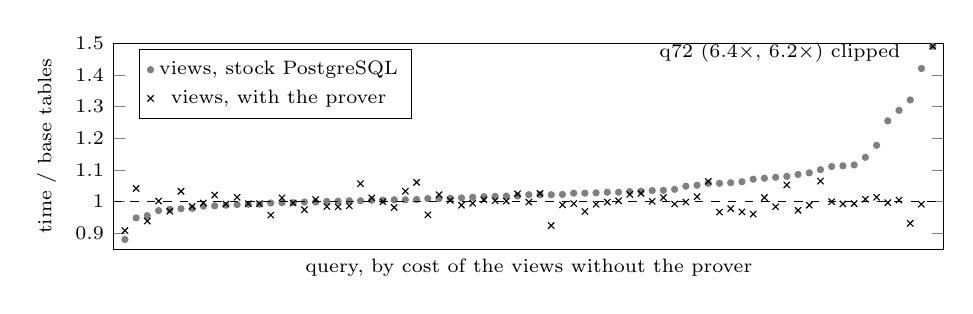
\begin{tikzpicture}
\begin{axis}[width=\columnwidth, height=4.2cm, ymin=0.85, ymax=1.5, xmin=0, xmax=74,
  xlabel={query, by cost of the views without the prover}, ylabel={time / base tables},
  xtick=\empty, ytick={0.9,1,1.1,1.2,1.3,1.4,1.5}, tick label style={font=\scriptsize},
  label style={font=\scriptsize}, legend style={font=\scriptsize, at={(0.03,0.97)}, anchor=north west},
  restrict y to domain=0:1.5, clip mode=individual]
\addplot[only marks, mark=*, mark size=1.1pt, gray] coordinates {(1,0.881) (2,0.949) (3,0.956) (4,0.972) (5,0.976) (6,0.978) (7,0.979) (8,0.986) (9,0.987) (10,0.989) (11,0.991) (12,0.992) (13,0.992) (14,0.996) (15,0.997) (16,0.997) (17,0.999) (18,0.999) (19,1.001) (20,1.002) (21,1.003) (22,1.003) (23,1.005) (24,1.005) (25,1.006) (26,1.006) (27,1.007) (28,1.010) (29,1.010) (30,1.011) (31,1.012) (32,1.014) (33,1.016) (34,1.017) (35,1.018) (36,1.018) (37,1.022) (38,1.022) (39,1.022) (40,1.023) (41,1.027) (42,1.027) (43,1.028) (44,1.030) (45,1.030) (46,1.032) (47,1.033) (48,1.035) (49,1.036) (50,1.039) (51,1.049) (52,1.052) (53,1.058) (54,1.058) (55,1.060) (56,1.063) (57,1.071) (58,1.074) (59,1.077) (60,1.080) (61,1.086) (62,1.091) (63,1.101) (64,1.111) (65,1.113) (66,1.116) (67,1.140) (68,1.178) (69,1.255) (70,1.288) (71,1.321) (72,1.420) (73,1.49)};
\addplot[only marks, mark=x, mark size=1.6pt, black] coordinates {(1,0.909) (2,1.042) (3,0.939) (4,1.002) (5,0.970) (6,1.033) (7,0.985) (8,0.996) (9,1.021) (10,0.993) (11,1.014) (12,0.994) (13,0.994) (14,0.958) (15,1.012) (16,0.996) (17,0.975) (18,1.007) (19,0.985) (20,0.984) (21,0.987) (22,1.057) (23,1.012) (24,1.000) (25,0.982) (26,1.033) (27,1.061) (28,0.959) (29,1.022) (30,1.004) (31,0.989) (32,0.995) (33,1.006) (34,1.003) (35,1.002) (36,1.025) (37,0.999) (38,1.026) (39,0.925) (40,0.990) (41,0.994) (42,0.969) (43,0.992) (44,0.999) (45,1.003) (46,1.023) (47,1.026) (48,1.001) (49,1.013) (50,0.993) (51,0.999) (52,1.016) (53,1.064) (54,0.967) (55,0.978) (56,0.968) (57,0.961) (58,1.013) (59,0.984) (60,1.053) (61,0.973) (62,0.989) (63,1.065) (64,1.000) (65,0.993) (66,0.994) (67,1.008) (68,1.014) (69,0.997) (70,1.005) (71,0.932) (72,0.992) (73,1.49)};
\legend{{views, stock PostgreSQL},{views, with the prover}}
\draw[dashed] (axis cs:0,1) -- (axis cs:74,1);
\node[font=\scriptsize, anchor=east] at (axis cs:71,1.47) {q72 ($6.4\times$, $6.2\times$) clipped};
\end{axis}
\end{tikzpicture}
\caption{TPC-DS at scale factor~10 through views that restate each history-keeping dimension
with its current attributes: run time of the 73 queries that read one, relative to the same query
on the base tables.}
\label{fig:views}
\end{figure}

\paragraph*{Views over versioned data} Reporting layers often show historical facts together with current
attributes. To test this pattern, we offered each history-keeping dimension of TPC-DS as a view of the same name. For
\sql{item}, the view is
\sql{SELECT h.*, c.i\_brand AS cur\_i\_brand, \ldots\ FROM item h LEFT JOIN item c ON c.i\_item\_id = h.i\_item\_id AND
c.i\_rec\_end\_date IS NULL}. We ran the unchanged queries through these views, with the five keys of current versions
declared, and compared them with the queries on the base tables (Fig.~\ref{fig:views}). At scale factor~10, the 73 queries
that read such a dimension contain 141 joins added by the views. Stock PostgreSQL keeps all of them, and the prover
removes all of them, with identical results. Query q72 is an exception: the view's \sql{FROM} list prevents it from being
flattened, whether or not the join is removed. It is fast again with \sql{from\_collapse\_limit} set to 20. Without q72,
the views cost 7\% with stock PostgreSQL ($836$ against $783$\,s), and nothing with the prover ($778$\,s). At scale
factor~1, they cost 2\%, or 17\% with q6, whose time the views raise from 29 to 48\,s. The joins are removed whatever
their size, but what they cost depends on the dimension. TPC-DS dimensions are small next to its facts: at scale
factor~10, \sql{item} has 102{,}000 rows and \sql{store\_sales} 28.8 million.


\ifextended
\subsection{Recommendation}\label{sec:exp-rec}


\paragraph*{Would a recommender find them?} We hid the declared indexes and generated candidate conditions from two
sources. The schema proposes \sql{IS [NOT] NULL} on nullable columns, boolean values, and the constants of columns
that look like a status, type or kind. The workload contributes the atoms that its queries apply, with their constants.
Of the 168 declared conditions on plain columns, half (84) only exclude \nul\ keys and follow from the key itself. Of the
other 84, the schema recovers 78, at the level of column and kind of atom, since the constants come from the data. The
workload recovers 68 with their constants, and both sources together recover 79. The misses are conditions that require
a non-empty string (\sql{<> ''}), and two predicates that our parser does not read. On the tables with these indexes, the
schema proposes 2{,}776 candidate atoms and the workload 524. The workload is thus the sharper source, and the schema the
broader one. Choosing keys under these conditions needs data, which these applications do not publish. We leave this to
deployments with real instances.

\paragraph*{Stability under updates} We mined the 15 dimension tables of TPC-DS at scale factor~1. We found 11{,}988
keys of at most three columns under conditions of at most two atoms, 10{,}645 of them conditional. We kept the 4{,}002
that also hold at scale factor~10. DuckDB's generator produces no refresh sets, so we emulated the dimension maintenance
of the specification on scale factor~1, in three rounds. In each round, 5\% of the current versions of the
history-keeping dimensions get a successor version, 5\% of the rows of the other maintained dimensions are updated in
place, and 2.5\% new entities are added. New attribute values are drawn from the existing values of each column. After
three rounds, 79\% of the 3{,}126 conditional keys on maintained tables that held at both scale factors still hold. Of
those that held at scale factor~1 only, 58\% still hold. Mined keys without conditions fare worse (45\% and 26\%), as they
are mostly accidents of small tables. The keys on the seven static dimensions all hold. Holding at a second scale factor
is therefore a useful but weak filter. Of the keys it keeps, 79\% survive, against 64\% of all conditional keys, but it
keeps only 36\% of the keys that survive. The emulation samples columns independently, so it breaks correlations that the
real generator keeps. These rates are therefore lower bounds.

\paragraph*{A public dataset} We used the Stack Exchange data of \sql{stats.stackexchange.com} from April 2024, with
5.6M rows in 8 tables. The schema proposed 457 conditions: values of type, status and flag columns, \nul\ tests, and
conjunctions of one of each. HPIValid found the keys of at most three columns on each scope, under both semantics. This
gave 107 recommendations in 147\,s. Under $\U{}$, a column that is \nul\ throughout a scope is trivially a key. Requiring
50 rows where the key is not \nul\ removed 46 such candidates. We also mined the data before 2020, and 97 of the 103
recommendations that carry dates still hold in 2024.

By our reading, 81 recommendations state invariants of the platform. A revision has one history row per kind of
change. A post has one initial body, title and tag set, and at most one vote that accepts an answer. An answer is
accepted by at most one question, which is a $\Ueq{}$ key among values that are not \nul. Two posts are linked once per
type of link. A user earns a tag badge once per class. The other 26 recommendations follow correlations, such as
licence versions that follow time. The hold-out data rejects only 2 of them, together with 4 invariants that turned out
to be false: a post can become community wiki, or a hot network question, twice.

All Stack Exchange sites share the same schema. We therefore checked the 101 recommendations that hold in 2024 on three
other sites (dba, academia and travel, with 0.5M posts). Of the 99 that can be tested, 86 hold on all three. The 13 that
fail include 7 of the 24 correlations, and 6 that we had read as invariants. A post can be protected or tweeted twice,
and on some sites it can receive several spam votes. Other sites are thus a sharper filter than later data. But the 17
correlations that pass follow the platform's history, which all sites share. Choosing among recommendations remains a
decision for the owner of the schema.

\paragraph*{Keys from data} By Proposition~\ref{prop:reduce}, an existing algorithm for unique column combinations
finds the keys under a fixed condition. We took seven real tables with 21 conditions each, under both semantics, which
gives 288 scopes that are not trivial. HyUCC and HPIValid of Desbordante~\cite{Desb} returned the same minimal keys as our
miner on every scope where our miner finished within 20\,s. HPIValid took $0.1$ to $61$\,ms per table in the median
(Appendix~\ref{app:disc}).
\else
\subsection{Where the keys come from}\label{sec:exp-rec}\label{sec:discovery}

Stack Exchange and TPC-DS declare no filtered unique indexes, so we recommended some. A recommendation consists of a
condition and a key. Conditions come from the schema, such as \nul\ tests and the values of columns that look like a
status or type, and from the workload. Under a fixed condition, the minimal keys are the minimal unique column
combinations of the rows that match it, after each \nul\ is replaced by a value of its own for $\U{}$, or all \nul s by
one value for $\Ueq{}$. Any algorithm for unique column combinations~\cite{PN17,BBFNPS20} therefore finds conditional keys. When
we hid the declared indexes of the ten applications, the schema recovered 78 of the 84 conditions that do more than
exclude \nul\ keys.

On \sql{stats.stackexchange.com}, HPIValid~\cite{Desb} found 107 recommendations in 147\,s. By our reading, 81 of them
state invariants of the platform, for example that an answer is accepted by at most one question. The other 26 follow
correlations in the data. On TPC-DS, we kept the 4{,}002 mined keys that hold at scale factors 1 and 10. After three
rounds of emulated maintenance, 79\% of the conditional ones on maintained tables still hold. The extended
version~\cite{EXT} describes the miners and these experiments in detail.
\fi


%=====================================================================
\section{Related Work}\label{sec:related}
%=====================================================================

\paragraph*{Uniqueness in optimisation} Semantic query optimisation rewrites queries using integrity
constraints~\cite{King81,CGM90}. Filtered unique indexes are such constraints, and the question is which rewrites they
allow. PostgreSQL first answered this question unsoundly, and then not at all (bug \#17975). Rowley proposed the
distinction between base restrictions and join clauses that we use for uniqueness, and it is under discussion for
estimates~\cite{Yan26}. Paulley and Larson~\cite{PL94} derive the uniqueness of query results from keys. Simmen et
al.~\cite{SSM96} and Neumann and Moerkotte~\cite{NM04} propagate functional dependencies for order optimisation, and
Kossmann et al.~\cite{KPN22} survey optimisation based on dependencies.\ifextended{} Godfrey et al.~\cite{GGZ01} exploit characterisations of the data that behave like constraints.\fi None of these works treats keys that hold on part of a table.
Deriving the keys of a join from those of its inputs goes back to Darwen~\cite{Dar92} and Paulley~\cite{Pau00}.
Section~\ref{sec:planner} adds what filtered keys need: a premise for each relation that holds under its own
restrictions, and a semantics ($\U$ or $\Ueq$) for each step.\ifextended{} The recommender of Section~\ref{sec:discovery} fits with lazy discovery of dependencies for
the optimiser, driven by the workload~\cite{KLNP22}.\fi

\paragraph*{Partial indexes} Stonebraker proposed partial indexes~\cite{Sto89}, and Seshadri and Swami generalised
them~\cite{SS95}. Later work concerns how to select them and how to use them as access paths. Choosing a partial index
for a query restriction is the implication test of predicate subsumption~\cite{LY85,GL01}. Using a partial \emph{unique}
index to prove uniqueness is an implication between constraints, which is what this paper decides.

\paragraph*{Declared but unenforced keys} DB2 eliminates joins using declared constraints~\cite{CGK99}. Snowflake,
Databricks and Oracle remove joins using primary and unique keys marked \sql{RELY}~\cite{RELYsf,RELYdb,RELYora}, and
Databricks also removes \sql{DISTINCT}. The system trusts such keys but does not check them. These keys hold on the whole
table and may be false. Filtered unique indexes, in contrast, are enforced but hold on part of a table. The question
is therefore not whether to trust them, but what they imply.

\paragraph*{Testing optimisers} Our differential testing follows the oracles for logic bugs of Rigger and
Su~\cite{RS20a,RS20b,RS20c}. We compare the planner with the rewrites off and on, and use mutants to show that the test
detects errors.

\paragraph*{Keys with nulls and conditions} Possible and certain keys~\cite{KLZ15,KLLZ16} and key
sets~\cite{Thalheim89,HLL11,HLL23} give keys a semantics for \nul. Here $\U{K}$ is the possible key. A certain key implies
$\Ueq{K}$, but filtered unique indexes cannot express it. Embedded uniqueness constraints~\cite{WLL19} and contextual
keys~\cite{WLL17} restrict keys by completeness or by context. CFDs~\cite{BFGJK07,FGJK08}, and extended CFDs with
disjunction and inequality~\cite{BFGM08}, bind functional dependencies to patterns over complete relations. Over complete
relations that are sets, a conditional key with a constant condition is a CFD. What our model adds is \nul\ in conditions
and keys, which is what filtered indexes mostly state. The hardness of Theorems~\ref{thm:dom} and~\ref{thm:neq} comes from
the same effect of finite domains that makes CFD implication coNP-complete, whereas it is polynomial over infinite
domains~\cite{FGJK08}.
Here, \nul\ against a value, and an \sql{IN}-list, act as a domain of two or three values. Discovery of unique column
combinations~\cite{PN17,BBFNPS20,AGN15} and of CFDs~\cite{FGLX11} informs our miner.


%=====================================================================
\section{Conclusion}\label{sec:conclusion}
%=====================================================================

A planner can trust a filtered unique index when it proves uniqueness from the table's own restrictions, all its
unique indexes and its \sql{CHECK} constraints, under the \nul\ semantics of the rewrite. For the predicates of almost all
real decisions, join-shaped rewrites can then be decided in polynomial time. Under the same conditions, group-shaped
rewrites are hard only through nullable columns that the query leaves open.

A prover built on these results fits into PostgreSQL's planner with 38 changed lines, and into CockroachDB's with 4. It
adds tens of microseconds to planning in the median. It allowed exactly what real catalogs imply, and it changed no
result on 1{,}000{,}000 random queries. What it gains depends on who writes the queries. Application code and reports use filtered
keys for integrity, and gain little. Users' queries over Stack Exchange gain up to $3.3\times$, mostly through keys
carried through joins. Views over versioned data lose every join they add.

Some limits remain. Range predicates and expression keys are not translated, and derived tables are not reasoned about.
Self-join elimination is not yet connected to the prover, because it needs the clauses that established uniqueness.


\ifextended
\appendices
\section{Proofs for Reasoning}\label{app:reason}

\begin{proof}[Proof of Theorem~\ref{thm:neq}, cases on $K$]
Both cases reduce from CNF satisfiability with \sql{NOT NULL} columns $A_1,\dots,A_n,B$ and the goal
$\{\tau\}:\U{A_1\cdots A_nB}$, so a violating pair shares a value $v_i$ on each $A_i$ (``$x_i$ is
true'' iff $v_i=1$). For ${\notin}$: $\tau$ has $\any$ everywhere, and clause constraints
$\{\rho\}:\U{B}$ have $\rho(A_i)={\notin}\{1\}$ for a positive and ${\notin}\{0\}$ for a negative
literal; the entry fails iff the literal is true, and a value other than 0, 1 makes no literal
true. For ${\in}$: $\tau(A_i)={\in}\{0,1\}$, and $\rho(A_i)={\in}\{0\}$ for a positive and
${\in}\{1\}$ for a negative literal.
\end{proof}

\begin{proposition}\label{prop:multi}
Deciding $\Sig\models\{\tpl{}\}:\U{B}$, and $\Sig\models\{\tpl{}\}:\Ueq{B}$, is coNP-complete already
when $\Sig$ consists of a single constraint whose condition is built from \sql{IS NULL},
\sql{IS NOT NULL}, \sql{AND} and \sql{OR}.
\end{proposition}

\begin{proof}
Membership in coNP follows from Lemma~\ref{lem:pairs}. Hardness is by reduction from CNF satisfiability with clauses
$c_1,\dots,c_m$ over $x_1,\dots,x_n$: take nullable columns $A_1,\dots,A_n$ and $B\in\NN$, read
``$A_i$ is not \nul'' as ``$x_i$ is true'', and let $\Sig=\{C:\U{B}\}$, where $C$ has one template
per clause $c_j$, with $\bot$ on $A_i$ if $x_i$ occurs positively in $c_j$ and $\top$ if negatively:
a record matches it iff its assignment falsifies $c_j$. A pair violating the goal agrees on $B$
and satisfies $\Sig$ iff one of its records lies outside the scope of $C$, that is, satisfies the
CNF. Hence $\Sig\models\varphi$ iff the CNF is unsatisfiable. As $B\in\NN$, the same holds for
$\Ueq{B}$.
\end{proof}

\paragraph*{Separations} Let $\sigma=\{\tpl{d{:}\,\bot}\}:\U{k}$ over columns $k,d$, and suppose a set
$\Sig$ of embedded uniqueness constraints $E:U$ (records total on $E$ are unique on $U\subseteq E$)
were equivalent to it. The table $A$ with two records $(k{:}\,1,d{:}\,\nul)$ violates $\sigma$, so it
violates some $E:U$ in $\Sig$, with $d\notin E$ as both records are \nul\ on $d$. The table $B$ with
$(k{:}\,1,d{:}\,\nul)$ and $(k{:}\,1,d{:}\,1)$ satisfies $\sigma$ but violates $E:U$, as $E\subseteq\{k\}$.
For $\sigma=\{\tpl{s{:}\,{\in}\{c\}}\}:\U{k}$ take $A$ with two records $(k{:}\,1,s{:}\,c)$ and $B$ with
two records $(k{:}\,1,s{:}\,c')$: both are total and duplicate, so every embedded constraint that $A$
violates $B$ violates too, while $B$ satisfies $\sigma$. For CFDs, two identical records satisfy
every CFD and violate every conditional \sql{UNIQUE} whose scope contains them; a single record
with $A=a$ and $B\neq b$ violates the CFD $(A=a\rightarrow B=b)$ and satisfies every conditional
\sql{UNIQUE}.

\section{Proof of the Determination Lemma}\label{app:det}

Fix a database that satisfies the constraints, and two rows $u,v$ of the join of the block that
agree on $G$, \nul\ equal to \nul. A row of the join consists of one part per relation outside
the inner sides of semi- and anti-joins: a row of the relation, at a position of its own, or
\nul s if an outer join null-extended it. We show by induction on the order in which relations
become determined that $u$ and $v$ have the same part of each determined relation $S$.

\emph{Entered through $G$.} $S$ is unique with \nul\ equal to \nul\ on its columns $K$ in $G$
among its rows that pass its restrictions and \sql{CHECK} constraints, and no outer join can
null these columns. So the parts of $S$ in $u$ and $v$ are rows of $S$, not \nul s; both pass the
restrictions, which are applied below every join; they agree on $K$ with \nul\ equal to \nul,
because $u$ and $v$ agree on $G$; hence they are the same row.

\emph{Entered through an equivalence class.} A column $s$ of $S$ is in an equivalence class with
two or more members, one of them a column $x$ of a determined relation $R$ or a column of $G$ that
no outer join nulls. The class's equalities are strict and applied wherever both columns are
available, so in every row that contains a row of $S$, its $s$ is the value of $x$ and not \nul.
By the induction hypothesis (or because $u$ and $v$ agree on $G$), $x$ is the same in $u$ and $v$.
If both contain a row of $S$, the two rows pass $S$'s restrictions and agree on all columns by
which $S$ was entered, with values, so $\U{}$ uniqueness of $S$ on them makes them one row. It
remains that both contain a row of $S$ or neither does. If no outer join can null $S$, both do.
Otherwise $S$ lies on the nullable side of left joins, and the rule requires each of their outer
sides to be determined: whether the nullable side of such a join is matched or null-extended is
a function of the outer row, which is the same in $u$ and $v$, and of the database, which is
fixed.

\emph{Entered through an outer join clause.} The clause equates a column $s$ of $S$, on the
nullable side, with a column $x$ of a determined relation on the outer side, and the whole outer
side is determined. Given the outer row, which $u$ and $v$ share, the rows of $S$ that the
clause admits pass $S$'s restrictions and have $s$ equal to the value of $x$; by $\U{}$
uniqueness at most one does. So both $u$ and $v$ contain it, or both are null-extended, as
whether a match exists depends on the outer row and the fixed database only.

Inner sides of semi- and anti-joins contribute no part and no row: a row of the join is
determined by its parts outside them. If every other relation is determined, $u$ and $v$ have
the same part of every relation, hence are the same combination of rows at the same positions,
that is, the same row of the join; so no two rows agree on $G$. For \sql{GROUP BY} with
aggregates, a relation $S$ determined by the remaining grouping columns $G'$ has the same part in
all rows of a group of $G'$, so its grouping columns do not split groups; $G'$ is kept non-empty,
since grouping by nothing yields a row even for an empty input. \qed

\section{The Axiomatisation}\label{app:axiom}

Fix the set $\Gamma$ of constants of an instance. The
\emph{profile} of a record has, per column, \nul, a constant of $\Gamma$, or $*$ for a value
outside $\Gamma$; it is the scope of exactly one template $\tau_p$, with ${\in}\{c\}$, $\bot$ and
${\notin}\Gamma$ as entries. For a goal with key part $\kappa$ (that is, $\U{K}$ or $\Ueq{K}$) and two
profiles $p,q$, let $c_\kappa(p,q)$ be the \emph{canonical pair}: records of profiles $p$ and $q$
that agree on $K$ and carry different fresh values wherever both have $*$ outside $K$; the
\emph{cell} $(p,q)$ is vacuous if no pair of these profiles agrees on $K$. Writing $\top$ for
${\notin}\emptyset$, $D$ for a condition, $\tau[A{\mapsto}e]$ for $\tau$ with entry $e$ on $A$, and
dropping templates with $\bot$ on a \sql{NOT NULL} column:
\begin{center}\small
\begin{tabular}{@{}l@{\ }l@{}}
(T) & ${}\Rightarrow\emptyset:\kappa$\\
(S) & $(D\cup\{\tau[A{\mapsto}\top],\tau[A{\mapsto}\bot]\}):\kappa$\\
 & \quad${}\Rightarrow(D\cup\{\tau[A{\mapsto}\any]\}):\kappa$\\
(V) & $(D\cup\{\tau[A{\mapsto}{\notin}S{\cup}\{c\}],\tau[A{\mapsto}{\in}\{c\}]\}):\kappa$\\
 & \quad${}\Rightarrow(D\cup\{\tau[A{\mapsto}{\notin}S]\}):\kappa$\\
(I) & $(D\cup\{\tau[A{\mapsto}{\in}\{c\}]:c\in S\}):\kappa$\\
 & \quad${}\Rightarrow(D\cup\{\tau[A{\mapsto}{\in}S]\}):\kappa$\\
(P) & $(D\cup\{\tau\}):\kappa,\ (D\cup\{\tau'\}):\kappa,\ \{\tau,\tau'\}:\kappa$\\
 & \quad${}\Rightarrow(D\cup\{\tau,\tau'\}):\kappa$\\
(C1) & $\sigma\Rightarrow\{\tau_p\}:\kappa$\quad if $c_\kappa(p,p)$ violates $\sigma$\\
(C2) & $\{\tau_p\}:\kappa,\ \{\tau_q\}:\kappa,\ \sigma\Rightarrow\{\tau_p,\tau_q\}:\kappa$\\
 & \quad if $c_\kappa(p,q)$ violates $\sigma$
\end{tabular}
\end{center}
In (S) the second template is omitted on a \sql{NOT NULL} column, in (V) $c\notin S$, and in
(C1), (C2) $\sigma$ is any constraint with constants in $\Gamma$, omitted when the cell is vacuous.

\begin{theorem}[Axiomatisation]\label{thm:axiom}
The rules (T), (S), (V), (I), (P), (C1) and (C2) form a sound and complete $3$-ary inference
system for the implication of conditional \sql{UNIQUE} constraints with conditions built from
\sql{=}, \sql{<>}, \sql{IN}, \sql{NOT IN}, \sql{IS [NOT] NULL}, \sql{AND} and \sql{OR}, under both
\nul\ semantics and any mix of them.
\end{theorem}

The proofs below use the following notation. Values come from an infinite domain $\mathbb V$. We write $\top$ for ${\notin}\emptyset$, drop
templates with $\bot$ on a column of $\NN$ (their scope is empty), and write $\scope(C)$ for the
records matching a condition $C$ and $\consts(\cdot)$ for the constants occurring in entries.
For a key part $\kappa$ with key $K$, records $t,t'$ \emph{agree under $\kappa$}, $t\ag_\kappa t'$,
if for all $A\in K$: $t[A]=t'[A]\neq\nul$ (for $\U{K}$), respectively $t[A]=t'[A]$ with \nul\ equal
to \nul\ (for $\Ueq{K}$). A pair $(t,t')$ \emph{violates} $C:\kappa$ if $t,t'\in\scope(C)$ and
$t\ag_\kappa t'$; this is symmetric in $t,t'$.

\subsection{Profiles and cells}

Fix a finite $\Gamma\subseteq\mathbb V$. A \emph{$\Gamma$-profile} $p$ assigns to each column an
element of $\Gamma\cup\{*,\bot\}$, and not $\bot$ to a column of $\NN$. The profile $\prof(t)$ of a
record has $t[A]$ where $t[A]\in\Gamma$, $\bot$ where $t[A]=\nul$, and $*$ otherwise; the template
$\tau_p$ has ${\in}\{c\}$ where $p$ has $c$, $\bot$ where $p$ has $\bot$, and ${\notin}\Gamma$ where $p$
has $*$. A profile $p$ \emph{matches} $\tau$ if every record of profile $p$ does, and $\Prof(C)$ is
the set of profiles matching a template of $C$.

\begin{lemma}[Profiles]\label{lem:profiles}
(a) $\scope(\tau_p)=\{t:\prof(t)=p\}$. (b) If $\consts(\tau)\subseteq\Gamma$, whether $t$ matches
$\tau$ depends only on $\prof(t)$; so $\scope(C)=\biguplus_{p\in\Prof(C)}\scope(\tau_p)$ when
$\consts(C)\subseteq\Gamma$.
\end{lemma}

\begin{proof}
(a) holds by definition. (b) On a column $A$, $t[A]$ matches $\any$ always, $\bot$ iff
$\prof(t)(A)=\bot$, ${\in}S$ with $S\subseteq\Gamma$ iff $\prof(t)(A)\in S$, and ${\notin}S$ with
$S\subseteq\Gamma$ iff $\prof(t)(A)\notin S\cup\{\bot\}$, as a value outside $\Gamma$ lies outside
$S$. Profile scopes are disjoint by (a).
\end{proof}

The cell $(p,q)$ is \emph{vacuous for $\kappa$} if some $A\in K$ has $p(A)\neq q(A)$, or
$p(A)=q(A)=\bot$ and $\kappa=\U{K}$. Otherwise the \emph{canonical pair} $c_\kappa(p,q)=(t_1,t_2)$
has, on $A\in K$, $t_1[A]=t_2[A]$ equal to $p(A)$ if $p(A)\in\Gamma$, to \nul\ if $p(A)=\bot$, and to a
value $v_A\notin\Gamma$ if $p(A)=*$; on $A\notin K$, the constant or \nul\ that each profile
prescribes, and where it has $*$ a value $u^i_A\notin\Gamma$; all of $v_A,u^1_A,u^2_A$ are distinct.
Then $\prof(t_1)=p$, $\prof(t_2)=q$ and $t_1\ag_\kappa t_2$, and a cell is vacuous iff no records of
profiles $p,q$ agree under $\kappa$.

\begin{lemma}[Weakest pair]\label{lem:weakest}
Let $(p,q)$ be non-vacuous for $\kappa$ and $\consts(\sigma)\subseteq\Gamma$. If $c_\kappa(p,q)$
violates $\sigma$, so does every pair $(t,t')$ with $\prof(t)=p$, $\prof(t')=q$ and $t\ag_\kappa t'$.
\end{lemma}

\begin{proof}
Let $\sigma=D:\lambda$ with key $L$ and $c_\kappa(p,q)=(t_1,t_2)$. By
Lemma~\ref{lem:profiles}(b), $t,t'\in\scope(D)$ as $t_1,t_2$ are. Let $A\in L$, where $t_1,t_2$
agree under $\lambda$. If $A\in K$: for $p(A)=q(A)=\bot$, $\kappa$ is $\Ueq{K}$, $t_1[A],t_2[A]$ are
\nul, so $\lambda$ is $\Ueq{L}$ and $t[A]=t'[A]=\nul$ agree; for a constant, $t[A]=t'[A]$ is that
constant; for $*$, $t[A],t'[A]$ are values made equal by $t\ag_\kappa t'$. If $A\notin K$: were
$p(A)=*$ or $q(A)=*$, $t_1[A],t_2[A]$ would be different and not both \nul, contradicting their
agreement; so $t[A]=t_1[A]$ and $t'[A]=t_2[A]$ are prescribed by the profiles, and agree.
\end{proof}

\begin{lemma}[Cells]\label{lem:cells}
Let $\varphi=C_\varphi:\kappa$ and $\Gamma\supseteq\consts(\Sig\cup\{\varphi\})$. Then $\Sig\models\varphi$
iff for all $p,q\in\Prof(C_\varphi)$ with $(p,q)$ non-vacuous, some $\sigma\in\Sig$ is violated by
$c_\kappa(p,q)$.
\end{lemma}

\begin{proof}
($\Leftarrow$) If $r$ satisfies $\Sig$ and $(t,t')$ in $r$ violates $\varphi$, then
$p=\prof(t),q=\prof(t')\in\Prof(C_\varphi)$, $(p,q)$ is non-vacuous, and the $\sigma$ violated by
$c_\kappa(p,q)$ is violated by $(t,t')$ (Lemma~\ref{lem:weakest}). ($\Rightarrow$) If no
$\sigma\in\Sig$ is violated by $c_\kappa(p,q)=(t_1,t_2)$ for a non-vacuous cell, the table
$\{t_1,t_2\}$ respects $\NN$, satisfies $\Sig$ (its pairs are $(t_1,t_2)$ and $(t_2,t_1)$) and violates
$\varphi$.
\end{proof}

\subsection{Soundness and completeness}

\begin{proof}[Proof of soundness]
(T): the empty condition has empty scope. (S), (V), (I): premise and conclusion have the same
key part and scope, since on $A$ the entries of the premise partition the records matching
the entry of the conclusion ($\top$ and $\bot$ for $\any$, only $\top$ on a \sql{NOT NULL} column;
${\notin}S{\cup}\{c\}$ and ${\in}\{c\}$ for ${\notin}S$; the ${\in}\{c\}$ for ${\in}S$). (P): let
$(t,t')$ violate the conclusion and $X=\scope(D)$. If both lie in $X\cup\scope(\tau)$ or both in
$X\cup\scope(\tau')$, a premise is violated; otherwise one lies in $\scope(\tau')\setminus X$ and the
other in $\scope(\tau)\setminus X$, violating $\{\tau,\tau'\}:\kappa$. (C1): a violating pair of
$\{\tau_p\}:\kappa$ has both profiles $p$ (Lemma~\ref{lem:profiles}(a)) and agrees, so $(p,p)$ is
non-vacuous and the pair violates $\sigma$ (Lemma~\ref{lem:weakest}). (C2): a violating pair with
equal profiles violates a premise $\{\tau_p\}:\kappa$ or $\{\tau_q\}:\kappa$; otherwise, up to symmetry,
its profiles are $p,q$ and it violates $\sigma$.
\end{proof}

For a template $\tau$ with $\consts(\tau)\subseteq\Gamma$ let $T(\tau)$ be the set of $\tau_p$ with $p$
matching $\tau$, and $\mu(\tau)=\sum_A\mu(\tau(A))$ with $\mu(\any)=|\Gamma|+2$,
$\mu({\notin}S)=|\Gamma\setminus S|$, $\mu({\in}S)=|S|-1$, $\mu(\bot)=0$; $\mu(\tau)=0$ iff $\tau$ is a
profile template.

\begin{lemma}[Merging]\label{lem:merge}
From $(D\cup T(\tau)):\kappa$, rules (S), (V), (I) derive $(D\cup\{\tau\}):\kappa$.
\end{lemma}

\begin{proof}
Induction on $\mu(\tau)$; for $\mu(\tau)=0$, $T(\tau)=\{\tau\}$. Otherwise choose $A$ with
$\mu(\tau(A))>0$ and the premise templates $\tau_1,\dots,\tau_k$ of the rule whose conclusion
template is $\tau$: $\tau[A{\mapsto}\top]$ and, off $\NN$, $\tau[A{\mapsto}\bot]$ if $\tau(A)=\any$;
$\tau[A{\mapsto}{\notin}S{\cup}\{c\}]$, $\tau[A{\mapsto}{\in}\{c\}]$ for some $c\in\Gamma\setminus S$ if
$\tau(A)={\notin}S$; $\tau[A{\mapsto}{\in}\{c\}]$, $c\in S$, if $\tau(A)={\in}S$ with $|S|\ge2$. Then
$\mu(\tau_i)<\mu(\tau)$ and $T(\tau)=T(\tau_1)\uplus\dots\uplus T(\tau_k)$. With
$E_i=D\cup\{\tau_1,\dots,\tau_i\}\cup T(\tau_{i+1})\cup\dots\cup T(\tau_k)$, the induction hypothesis
derives $E_i:\kappa$ from $E_{i-1}:\kappa$, and the rule turns $E_k:\kappa$ into $(D\cup\{\tau\}):\kappa$.
\end{proof}

\begin{proof}[Proof of completeness]
Let $\Sig\models\varphi=C_\varphi:\kappa$, $\Gamma=\consts(\Sig\cup\{\varphi\})$; if $C_\varphi=\emptyset$ use (T).
Let $P=\Prof(C_\varphi)$ and $T_P=\{\tau_p:p\in P\}=\bigcup_{\theta\in C_\varphi}T(\theta)$.
(1)~For $p\in P$, (C1) derives $\{\tau_p\}:\kappa$, with the premise that Lemma~\ref{lem:cells}
provides if $(p,p)$ is non-vacuous. (2)~For $p\neq q$ in $P$, (C2) derives
$\{\tau_p,\tau_q\}:\kappa$ likewise. (3)~For $Q\subseteq T_P$ with $|Q|\ge3$, by induction on $|Q|$, (P)
with distinct $\tau,\tau'\in Q$ and $D=Q\setminus\{\tau,\tau'\}$ derives $Q:\kappa$; so $T_P:\kappa$ is
derived. (4)~With $C_\varphi=\{\theta_1,\dots,\theta_m\}$ and
$F_j=\{\theta_1,\dots,\theta_j\}\cup T(\theta_{j+1})\cup\dots\cup T(\theta_m)$, Lemma~\ref{lem:merge}
derives $F_j:\kappa$ from $F_{j-1}:\kappa$; $F_0=T_P$ and $F_m=C_\varphi$.
\end{proof}

Every derived constraint has the goal's key part and members of $\Sig$ occur only as the $\sigma$ of
(C1) and (C2), so the rules are complete for each semantics alone. Derivations can be doubly
exponentially long ($|P|$ is exponential and step (3) uses all subsets), consistent with
coNP-hardness; the decision procedures of Section~\ref{sec:reasoning} do not search for
derivations.

\subsection{A derivation and a counterexample}

\begin{example}[A derived key]\label{ex:derivation}
A table has the filtered unique indexes
\begin{center}\small
\sql{UNIQUE (s) WHERE s = 'a'},\quad \sql{UNIQUE (s) WHERE s <> 'a'},\quad
\sql{UNIQUE ((1)) WHERE s IS NULL},
\end{center}
that is $\sigma_1=\{\tpl{s{:}\,{\in}\{a\}}\}:\U{s}$, $\sigma_2=\{\tpl{s{:}\,{\notin}\{a\}}\}:\U{s}$ and
$\sigma_3=\{\tpl{s{:}\,\bot}\}:\U{\emptyset}$ (at most one row with $s$ \nul). Together they
enforce \sql{UNIQUE NULLS NOT DISTINCT (s)}, $\varphi=\{\tpl{}\}:\Ueq{s}$, so \sql{SELECT DISTINCT s}
can drop its \sql{DISTINCT}. Here $\Gamma=\{a\}$ and the profiles are $a$, $*$ and $\bot$, with
templates $\tpl{s{:}\,{\in}\{a\}}$, $\tpl{s{:}\,{\notin}\{a\}}$ and $\tpl{s{:}\,\bot}$; the cells of
two different profiles are vacuous, as the profiles differ on the key $s$. Writing conditions
by their entries on $s$:
\begin{center}\small
\begin{tabular}{@{}r@{\ \ }l@{\ \ }l@{}}
1 & $\{{\in}\{a\}\}:\Ueq{s}$ & (C1), $\sigma_1$; $c(a,a)$: $s=a,a$\\
2 & $\{{\notin}\{a\}\}:\Ueq{s}$ & (C1), $\sigma_2$; $c(*,*)$: $s=v,v$\\
3 & $\{\bot\}:\Ueq{s}$ & (C1), $\sigma_3$; $c(\bot,\bot)$: $s=\nul,\nul$\\
4 & $\{{\in}\{a\},{\notin}\{a\}\}:\Ueq{s}$ & (C2), 1, 2; vacuous\\
5 & $\{{\in}\{a\},\bot\}:\Ueq{s}$ & (C2), 1, 3; vacuous\\
6 & $\{{\notin}\{a\},\bot\}:\Ueq{s}$ & (C2), 2, 3; vacuous\\
7 & $\{{\in}\{a\},{\notin}\{a\},\bot\}:\Ueq{s}$ & (P), 5, 6, 4; $D=\{\bot\}$\\
8 & $\{\top,\bot\}:\Ueq{s}$ & (V), 7; $S=\emptyset$, $c=a$\\
9 & $\{\any\}:\Ueq{s}$, i.e.\ $\varphi$ & (S), 8
\end{tabular}
\end{center}
Step 3 uses that two \nul s agree under $\Ueq{}$; the cell $(\bot,\bot)$ would be vacuous for a
$\U{}$ goal. Each $\sigma_i$ is needed: without it, its cell has no premise.
\end{example}

\begin{example}[A counterexample]\label{ex:counter}
Take the two scopes of Example~\ref{ex:mixed}: $\sigma_1=\{\tpl{d{:}\,\bot}\}:\Ueq{k}$,
$\sigma_2=\{\tpl{d{:}\,\top}\}:\U{k}$, and the goal $\varphi=\{\tpl{x{:}\,1}\}:\U{k}$, so $\Gamma=\{1\}$.
Following the proof of completeness, the cells within the scope of $\varphi$ are checked one by
one. The cell of $p=(k{:}\,*,d{:}\,\bot,x{:}\,1)$ and $q=(k{:}\,*,d{:}\,*,x{:}\,1)$ is non-vacuous
(both have a value on $k$), and its canonical pair is
\[
t_1=(k{:}\,v,\ d{:}\,\nul,\ x{:}\,1),\qquad t_2=(k{:}\,v,\ d{:}\,u,\ x{:}\,1).
\]
It violates neither premise: $t_2$ is outside the scope of $\sigma_1$ and $t_1$ outside that of
$\sigma_2$. So (C2) has no premise for this cell, the derivation cannot be completed, and by
Lemma~\ref{lem:cells} the table $\{t_1,t_2\}$ is a counterexample: it satisfies both indexes and
has two rows with $x=1$ and the same $k$. This is the evidence a planner obtains when it refuses
to drop a join probing $k$ among the rows with $x=1$.
\end{example}

\section{Discovery}\label{app:disc}

For a table $r$, let
$\mathrm{Th}(r)$ be the set of conditional \sql{UNIQUE} constraints that $r$ satisfies; a
\emph{cover} of $\mathrm{Th}(r)$ is a finite subset that implies all of it.

\begin{theorem}[Finite covers]\label{thm:cover}
Let $\Gamma$ be the constants occurring in $r$. The constraints $\{\tau_p,\tau_q\}:\kappa$ that hold on
$r$, for $\Gamma$-profiles $p,q$ and key parts $\kappa\in\{\U{K},\Ueq{K}\}$ with $K$ minimal, form a
finite cover of $\mathrm{Th}(r)$; it implies also the constraints with constants that do not
occur in $r$.
\end{theorem}

The cover is finite because \sql{NOT IN} names ``a value that $r$ does not contain'' with one
entry. But it shows that the unrestricted problem is degenerate: every value of $r$ lies in
$\Gamma$, so the profile of a row records all its values, and conditions can single out any set
of rows. The cover above enumerates pairs of rows---for tables of at most five rows and three
columns it has $146$ members in the median and up to $4{,}232$---and the largest scope on which
a key $K$ is unique is found trivially by keeping one row per value of $K$. Discovery is
meaningful only over a bounded condition language. Let $\mathcal L_a$ be the templates with at
most $a$ entries other than $\any$, each an \emph{atom} \sql{A = c}, \sql{A <> c} ($c$ in the
active domain of $A$), \sql{A IS NULL} or \sql{A IS NOT NULL}, and let $\mathrm{Disc}_a(r)$ list,
for every $\tau\in\mathcal L_a$ and both semantics, the minimal keys $K$ such that $\tau:\U{K}$,
respectively $\tau:\Ueq{K}$, holds on $r$. As a constraint implies the same constraint with a
larger key, $\mathrm{Disc}_a(r)$ covers the constraints with conditions in $\mathcal L_a$ that
hold on $r$.

\begin{theorem}[Complexity of discovery]\label{thm:disc}
Let $r$ be a table over $R$, and $d$ the largest active domain of a column.
\begin{enumerate}
\item[(a)] Whether a given constraint holds on $r$ is decidable in polynomial time.
\item[(b)] $|\mathcal L_a|\le\big(|R|\,(2d+3)\big)^a$, polynomial for fixed $a$.
\item[(c)] Given $\tau$ and $k$, deciding whether $\tau:\U{K}$ holds on $r$ for some $K$ with $|K|\le k$
  is NP-complete and, parameterised by $k$, W[2]-complete, already for $\tau=\tpl{}$; the same
  holds for $\Ueq{}$.
\item[(d)] For given $\tau$ and semantics, the minimal keys are the minimal transversals of a
  hypergraph on $R$ with at most $|r|^2$ edges, computable in polynomial time; for $\tau=\tpl{}$
  over tables without \nul, enumerating them is equivalent under parsimonious reductions to
  enumerating the minimal transversals of a hypergraph~\cite{BFS22}.
\end{enumerate}
Hence, for fixed $a$, $\mathrm{Disc}_a(r)$ is computable in incremental quasi-polynomial
time~\cite{FK96}, in output-polynomial time if minimal transversals can be enumerated in
output-polynomial time, and for $a=0$ only then~\cite{EG95}. With keys bounded by a fixed
size, it takes polynomial time.
\end{theorem}

Part (c) follows from the unconditional case~\cite{BFS22,SR92}, part (d) from the observation
that $K$ is a key within a scope iff it meets the set of columns on which every two rows of the
scope fail to agree (proofs below). Our miner works with $a=2$ and keys
of at most three columns, so its search is polynomial; what makes discovery hard is unbounded
key size, as for unconditional keys, not the conditions.

\paragraph*{Fixing the condition} By part (d) and Proposition~\ref{prop:reduce}, discovery for
a fixed condition is discovery of unique column combinations on the encoded rows in scope.
Algorithm~\ref{alg:fixc} follows the hybrid scheme of~\cite{PN17}: disagreement sets of
neighbouring rows in the position list indexes (PLIs) give candidate keys as minimal
transversals; each candidate is validated by intersecting PLIs, and a failing candidate yields
a pair whose disagreement set updates the candidates by one step of Berge's
algorithm~\cite{Ber89}, $\mathrm{Add}_k(T,D)=\min\big(\{X\in T:X\cap D\ne\emptyset\}\cup\{X\cup\{A\}:X\in
T,\,X\cap D=\emptyset,\,A\in D,\,|X|<k\}\big)$.

\begin{algorithm}[t]
\caption{$\textsc{FixC}(r,C,\kappa,k,H_0)$: minimal keys of at most $k$ columns}\label{alg:fixc}
\small
\begin{algorithmic}[1]
\State $S\gets$ the rows of $r$ matching $C$; \textbf{if} $|S|<2$ \textbf{return} $\{\emptyset\}$
\State replace each \nul\ in $S$ by a value of its own ($\U{}$) or by one value $\bot$ ($\Ueq{}$)
\State $\pi_A\gets$ clusters of $\ge2$ rows of $S$ equal on $A$, for each $A\in R$
\State $H\gets\{D\in H_0:\text{its two rows lie in }S\}\cup\{D(t,t'):t,t'\text{ consecutive in a cluster}\}$
\State $T\gets\{\emptyset\}$; \textbf{for each} $D\in\min H$: $T\gets\mathrm{Add}_k(T,D)$; \ $V\gets\emptyset$
\While{some $X\in T\setminus V$}
  \If{the refinement of $\pi$ by $X$ has a cluster with rows $t,t'$}
    \State \textbf{if} $D(t,t')=\emptyset$ \textbf{return} $\emptyset$ \Comment{no key exists}
    \State $H\gets H\cup\{D(t,t')\}$;\ \ $T\gets\mathrm{Add}_k(T,D(t,t'))$
  \Else\ $V\gets V\cup\{X\}$
  \EndIf
\EndWhile
\State \Return $T$ (and $H$, for reuse)
\end{algorithmic}
\end{algorithm}

\begin{algorithm}[t]
\caption{$\textsc{DiscA}(r,a,k)$: all templates of $\mathcal L_a$}\label{alg:disca}
\small
\begin{algorithmic}[1]
\For{$\kappa\in\{\U{},\Ueq{}\}$ and $\tau\in\mathcal L_a$ by increasing number of atoms}
  \State $\tau'\gets\tau$ without its last atom \Comment{a wider scope}
  \State $(K_\tau,H_\tau)\gets\textsc{FixC}(r,\{\tau\},\kappa,k,H_{\tau'})$ \Comment{$H_{\tpl{}}$ from $H_0=\emptyset$}
\EndFor
\State \Return all $\tau:\kappa(K)$ with $K\in K_\tau$
\end{algorithmic}
\end{algorithm}

\begin{proposition}\label{prop:fixc}
$\textsc{FixC}$ returns exactly the minimal keys of at most $k$ columns, and $\textsc{DiscA}$
returns $\mathrm{Disc}_a(r)$ restricted to such keys.
\end{proposition}

\begin{proof}
Every disagreement set in $H$ belongs to two rows of the scope, so every key meets it. A returned
$X$ is a validated key and a minimal transversal of $H$, so no proper subset of $X$ is a key. A
minimal key $K$ with $|K|\le k$ is a transversal of $H$ and contains a minimal one, $X$, with
$|X|\le k$, which $\mathrm{Add}_k$ keeps; $X$ is validated, so it is a key and $X=K$. Each failed
validation adds a set that the candidate misses, so $H$ grows and the loop ends. Inherited sets in
$\textsc{DiscA}$ are kept only if both rows lie in the narrower scope.
\end{proof}

The cost is dominated by validations, $O(|S|\,|X|)$ each; on random tables both procedures
agree with exhaustive search (Section~\ref{sec:exp-disc}).

\paragraph*{Fixing the key} Our second miner goes the other way. For a candidate key $K$
(at most three columns) the pairs of records that agree on $K$ are computed once by grouping; a
condition makes $C:\U{K}$ hold iff no such pair has both records in its scope, so all valid
templates of at most two atoms---a frequent constant of a low-cardinality column, a column
present, a column missing---are found in one pass over the atom sets the pairs share, and
single-constant templates are merged into \sql{IN}-lists whose cross pairs are
clean. Results implied by the declared indexes or by more general results are dropped
by the prover of Section~\ref{sec:planner}, so the recommendation is irredundant.

The difficulty is not search but accidental keys. On TPC-DS's six-row \sql{call\_center} table,
342 unconditional keys hold; checking them on a second scale factor keeps 156, and on small
dimension tables almost all. Ranking by scope size, identifier-like columns and simplicity of the
condition helps; a recommender should, in addition, prefer keys that the workload can use.

\subsection{Proofs}

\begin{proof}[Proof of Theorem~\ref{thm:cover}]
Every listed constraint holds on $r$ by definition, and there are finitely many, as there are
finitely many $\Gamma$-profiles and keys. Let $\varphi=C:\kappa$ hold on $r$, with key $K_\varphi$, and
suppose the cover $\Sig$ does not imply it. With $\Gamma'=\Gamma\cup\consts(\varphi)$,
Lemma~\ref{lem:cells} yields $\Gamma'$-profiles $p',q'\in\Prof(C)$ whose cell is non-vacuous and
whose canonical pair $(t_1,t_2)$ satisfies $\Sig$. Let $p,q$ be the $\Gamma$-profiles of $t_1,t_2$
and $Z\supseteq K_\varphi$ the set of columns on which $t_1,t_2$ agree under $\kappa$; write
$\kappa_Z$ for the key part of the same semantics with key $Z$. The pair $(t_1,t_2)$ violates
$\{\tau_p,\tau_q\}:\kappa_Z$. If that constraint held on $r$, so would one with a minimal key
$K\subseteq Z$, which belongs to $\Sig$ and is also violated by $(t_1,t_2)$---a contradiction. So
$r$ has rows $t,t'$ at different positions with $\Gamma$-profiles in $\{p,q\}$ that agree on $Z$
under $\kappa$. Rows of $r$ carry only values of $\Gamma$, so these profiles contain no $*$; hence
the corresponding record of the canonical pair carries only values of $\Gamma$ or \nul, and its
$\Gamma'$-profile, $p'$ or $q'$, equals its $\Gamma$-profile. Thus $t,t'$ have $\Gamma'$-profiles in
$\{p',q'\}\subseteq\Prof(C)$, lie in $\scope(C)$ by Lemma~\ref{lem:profiles}, and agree on
$K_\varphi\subseteq Z$ under $\kappa$: $(t,t')$ violates $\varphi$ on $r$, a contradiction.
\end{proof}

The construction was checked mechanically: on $400$ random tables and $2{,}000$ random
constraints, with constants inside and outside the tables, ``$\varphi$ holds on $r$'' coincided with
``the cover implies $\varphi$''.

\begin{proof}[Proof of Theorem~\ref{thm:disc}]
(a) Collect the rows of the scope, drop for $\U{K}$ those with \nul\ on $K$, and look for two rows
with equal projections on $K$ (with \nul\ as a value for $\Ueq{K}$) by sorting or hashing.
(b) A template of $\mathcal L_a$ chooses at most $a$ columns and, for each, one of at most $2d+2$
atoms; counting the choice ``no atom'' gives the bound.
(c) Membership in NP: guess $K$ and check it by (a). For hardness take $\tau=\tpl{}$ and tables
without \nul, on which $\U{K}$ and $\Ueq{K}$ both say that $K$ is a unique column combination.
Deciding whether a unique column combination of size at most $k$ exists is NP-complete and,
parameterised by $k$, W[2]-complete~\cite{BFS22}; finding a minimum one is NP-hard~\cite{SR92}.
(d) For rows $t,t'$ let $D_\kappa(t,t')$ be the set of columns on which they do not agree under
$\kappa$. Then $\tau:\kappa$ holds on $r$ iff $K\cap D_\kappa(t,t')\neq\emptyset$ for all rows $t,t'$ at
different positions in the scope of $\tau$, i.e.\ iff $K$ is a transversal of the hypergraph of
these sets; the minimal keys are its minimal transversals. If some set is empty, no key exists.
For $\tau=\tpl{}$ and tables without \nul\ these are the minimal unique column combinations, whose
enumeration is equivalent to transversal enumeration under parsimonious
reductions~\cite{BFS22}. For the consequences: $\mathrm{Disc}_a(r)$ consists of
$2|\mathcal L_a|$ transversal problems, each built in time $O(|r|^2|R|)$; the duality test of
Fredman and Khachiyan runs in quasi-polynomial time and, when it fails, returns a point from
which a new minimal transversal is obtained, so minimal transversals are enumerated in
incremental quasi-polynomial time~\cite{FK96}; an output-polynomial algorithm for transversals gives one for each problem and
hence for their union, whose output is the sum of theirs; for $a=0$ the converse holds as minimal
unique column combinations can be enumerated in output-polynomial time only if transversals
can~\cite{EG95,BFS22}. With $|K|\le k$ fixed, all $O(|R|^k)$ candidate keys are checked by (a)
for each template.
\end{proof}

\begin{proof}[Proof of Proposition~\ref{prop:reduce}]
After the replacement, two records agree on $K$ in the plain sense iff they agree under the
chosen semantics, so $C:\kappa(K)$ holds on $r$ iff $K$ is unique on the records matching $C$.
\end{proof}

\subsection{Experiments}\label{sec:exp-disc}

\paragraph*{Correctness} $\textsc{FixC}$ agreed with exhaustive search over all subsets of columns
on $5{,}000$ random tables of up to five columns and twelve rows with \nul s and duplicates, random
conditions with $=$, \sql{<>}, \sql{IN}, \sql{NOT IN} and \sql{IS [NOT] NULL}, both semantics and
key bounds $k\in\{1,2,\infty\}$, and on $1{,}500$ wider tables (four to eight columns, up to 40
rows) with up to 44 minimal keys each; $\textsc{DiscA}$ with inherited disagreement sets agreed with
$\textsc{FixC}$ from scratch on all $42{,}958$ templates of $\mathcal L_2$ over 500 random tables.
\paragraph*{Cost} On seven real tables (Table~\ref{tab:bench}) we ran $\textsc{FixC}$ for the empty
condition and 20 single-atom conditions (the most frequent constants, \texttt{IS NULL} and
\texttt{IS NOT NULL} of the sparsest columns), under both semantics, with keys of at most three
columns, against a level-wise baseline that validates every candidate whose subsets are not keys
(single-threaded Python, same PLIs, same output on all 294 runs). $\textsc{FixC}$ needs 6--85 times
fewer validations and is faster on 238 of the 294 runs, with median speed-ups of 1.6--5.7 on six
tables and up to 88 on UniProt. It loses on Hockey.Teams (median 0.35): with about 300 minimal keys
per condition, maintaining the transversals costs more than the validations it saves, which are
cheap on 1{,}519 rows. Inheriting disagreement sets in $\textsc{DiscA}$ (70--86 single-atom
templates per table) saved at most 13\% of the time against $\textsc{FixC}$ from scratch, and nothing
on most tables: the seeds from PLI neighbours already find most disagreement sets, and validation
dominates. Inheritance is therefore a minor optimisation.
\begin{table}[t]\centering\small\setlength{\tabcolsep}{3pt}
\caption{$\textsc{FixC}$ against level-wise validation, keys of $\le3$ columns: medians over 42 runs (21 conditions, two semantics); H.\,= Hockey, V.\,= VOC.}\label{tab:bench}
\begin{tabular}{@{}lrrrrrr@{}}\toprule
table & rows & cols & keys & \multicolumn{2}{c}{FixC ms (val.)} & levels ms (val.)\\\midrule
H.Master & 7{,}761 & 31 & 263 & 462 & (359) & 788 (2{,}268)\\
H.Coaches & 1{,}812 & 14 & 4 & 14 & (5) & 55 (427)\\
H.Teams & 1{,}519 & 27 & 310 & 704 & (356) & 204 (3{,}133)\\
H.Goalies & 4{,}278 & 23 & 46 & 101 & (53) & 420 (2{,}005)\\
V.voyages & 8{,}131 & 23 & 37 & 97 & (37) & 558 (1{,}094)\\
V.seafarers & 4{,}468 & 10 & 3 & 10 & (3) & 15 (73)\\
UniProt (20k) & 20{,}000 & 100 & 396 & 1{,}655 & (410) & 11{,}587 (24{,}744)\\\bottomrule
\end{tabular}\end{table}

\paragraph*{Against UCC algorithms} On the same seven tables and 21 conditions under both
semantics (288 scopes with at least two records; UniProt sampled to 20{,}000 of its rows), we
wrote each encoded scope to a file and ran HyUCC and HPIValid of Desbordante~2.4.1 (C++, one
thread)~\cite{Desb}. The two returned the same keys on all 288 scopes; $\textsc{FixC}$ without a
size bound returned them on the 236 it finished within 20\,s, and with at most three columns on
the 281 it finished. HPIValid took $0.1$--$61$\,ms per table in the median, HyUCC $0.4$--$50{,}091$\,ms:
under $\Ueq{}$ on UniProt, where the scopes have about 76{,}000 minimal keys in the median, HyUCC
needed up to 21 minutes. $\textsc{FixC}$ with keys of at most three columns took $6.4$ times as
long as HPIValid in the median, loading included. Widening UniProt from 10 to 100 columns raised
HPIValid from $0.5$ to $45$\,ms. Our contribution to discovery is the reduction, not a new
algorithm for unique column combinations.

Scaling the rows of the 30-column UniProt exports from 16{,}000 to 512{,}000 (empty condition and
three \texttt{IS [NOT] NULL} conditions, both semantics; 40 scopes) kept all answers equal.
HPIValid grew from $2.5$ to $54$\,ms and HyUCC from $18$ to $1{,}479$\,ms on the empty condition
under $\U{}$, while reading the file grew from $0.4$ to $16$\,s and dominated both. $\textsc{FixC}$
with keys of at most three columns needed $0.7$\,s at 16{,}000 rows and $16$\,s at 256{,}000, and
exceeded 20\,s at 512{,}000 on the large scopes.

On 40 of the LakeBench tables of Section~\ref{sec:exp-decisions}, cut to the miner's key columns and
up to 12 condition columns (1{,}630 scopes of up to 163{,}414 rows), all four agreed on every scope
and $\textsc{FixC}$ always finished; in the median per table HPIValid took $0.4$\,ms, HyUCC
$4.3$\,ms and $\textsc{FixC}$ with at most three columns $77$\,ms.

\section{Further Experiments}\label{app:exp}

\paragraph*{Scaling of the decision procedure} On 30-column schemas with random conditional keys
of one or two atoms, our Python implementation of the canonical-pair search needs $0.15$, $0.37$,
$2.2$ and $15$\,ms in the median for $|\Sig|=10$, $100$, $1{,}000$ and $10{,}000$ at $b=4$, against
$0.34$--$244$\,ms for a SAT encoding; for $|\Sig|=100$ it grows from $0.19$\,ms at $b=0$ to
$669$\,ms at $b=16$, where SAT stays at about $2$\,ms. The polynomial case of
Theorem~\ref{thm:pos} is the $b=0$ column.

\paragraph*{A rewrite layer outside the planner} A catalog-reading rewrite layer in Python reproduced all 2{,}588 decisions on the eight tables whose
indexes PostgreSQL can build (on UniProt some index rows exceed 8\,kB), and the 80 sampled
rewrites it emitted returned the original results. Reading a table's constraints took
1--11\,ms and deciding and rewriting a query $3.2$\,ms in the median in Python. The rewrites ran
$1.8\times$ (\sql{DISTINCT}) and $3.5\times$ (left join) faster in the median, and removing the
join $10.7$--$32.3\times$ on NCVoter. These runs used catalogs with all key classes of the
miner, not filtered unique indexes only.

\paragraph*{Mining the TPC-DS workload} The queries are also a source of conditions. The local
predicates of each table occurrence (conjuncts of \sql{WHERE} and inner-join \sql{ON} clauses on
that table alone, kept as SQL including ranges) give 162 distinct conditions on 22 tables in 96
of the 99 queries, extracted in $1.5$\,s. Checked by grouping at scale factors 1 and 10, 124 of
the 181 key demands of the queries---the columns a block joins, groups or semi-joins on---hold
under their condition, but 118 contain the primary key, and only 3 hold because of the
condition, all on scopes of two to four rows that the query parameters select. Running
$\textsc{FixC}$ under every condition on a dimension table (keys of at most two columns, 14\,s in
all) finds 1{,}983 keys that hold only under their condition, 1{,}382 of them also at scale
factor 10, and 844 of these on scopes of fewer than 100 rows. Of the 794 under conditions of
equalities and \sql{IN}-lists, 232 hold for every value of the condition columns---$d_{dom}$
within each month, for instance---and so are composite keys that include those columns
(here $(d_{year},d_{moy},d_{dom})$) rather than conditional ones; the others depend on the
parameter values. Mining the workload finds scopes cheaply, but a recommender needs a
significance filter, and the selective, parameterised predicates of a benchmark are not where
filtered unique indexes live.

\fi

% ICDE 2027 requires AI-generated content to be disclosed in the acknowledgements; this section
% does not count towards the 12 pages. The authors must check that it describes their use.
\section*{Acknowledgment}
Claude (Anthropic), through Claude Code, was used for this work. It generated text for the article, code for the PostgreSQL prover and CockroachDB port, experiment
scripts, random schema and query generators (Sections~\ref{sec:planner}
and~\ref{sec:experiments}); it ran the experiments, compiled their results, drew the tables and
figures, checked the reductions of Section~\ref{sec:reasoning} by brute force on random instances,
and reviewed drafts. The authors directed the work and are responsible for the correctness and
originality of the paper.

% The last page is balanced by a column break before reference 47 (extended) or 20 (submission).
% Re-check the numbers when the text or references move.
\ifextended\IEEEtriggeratref{47}\else\IEEEtriggeratref{20}\fi
\begin{thebibliography}{99}
\bibitem{AGN15} Z.~Abedjan, L.~Golab, F.~Naumann. Profiling relational data: a survey.
  \emph{VLDB J.} 24(4), 2015.
\ifextended
\bibitem{Ber89} C.~Berge. \emph{Hypergraphs: Combinatorics of Finite Sets}. North-Holland,
  1989.
\fi
\bibitem{BBFNPS20} J.~Birnick, T.~Bl\"asius, T.~Friedrich, F.~Naumann, T.~Papenbrock,
  M.~Schirneck. Hitting set enumeration with partial information for unique column combination
  discovery. \emph{Proc. VLDB Endow.} 13(11):2270--2283, 2020.
\ifextended
\bibitem{BFS22} T.~Bl\"asius, T.~Friedrich, M.~Schirneck. The complexity of dependency
  detection and discovery in relational databases. \emph{Theor. Comput. Sci.} 900:79--96,
  2022. % doi:10.1016/j.tcs.2021.11.020; KIT lists 2021, volume dated January 2022
\fi
\bibitem{BFGJK07} P.~Bohannon, W.~Fan, F.~Geerts, X.~Jia, A.~Kementsietsidis. Conditional
  functional dependencies for data cleaning. In \emph{ICDE}, pp.~746--755, 2007.
\bibitem{BFGM08} L.~Bravo, W.~Fan, F.~Geerts, S.~Ma. Increasing the expressivity of conditional
  functional dependencies without extra complexity. In \emph{ICDE}, pp.~516--525, 2008.
\bibitem{SchemaPile} T.~D\"ohmen, R.~Geacu, M.~Hulsebos, S.~Schelter. SchemaPile: a large collection of
  relational database schemas. \emph{Proc. ACM Manag. Data} 2(3), 172:1--172:25, 2024.
\bibitem{STATSCEB} Y.~Han, Z.~Wu, et al. Cardinality estimation in DBMS: a comprehensive
  benchmark evaluation. \emph{PVLDB}, 15(4):752--765, 2021.
\bibitem{Quarry} H.~Triedman. wikidb: queries from Wikimedia's Quarry. Hugging Face dataset
  \sql{htriedman/wikidb}, 2023.
\bibitem{SkyServer} A.~S.~Szalay, J.~Gray, et al. The SDSS SkyServer: public access to the Sloan
  Digital Sky Server data. In \emph{SIGMOD}, 2002.
\bibitem{SEDE} M.~Hazoom, V.~Malik, B.~Bogin. Text-to-SQL in the wild: a naturally-occurring
  dataset based on Stack Exchange data. In \emph{NLP4Prog Workshop at ACL}, 2021.
\bibitem{Desb} G.~Chernishev et al. Desbordante: from benchmarking suite to
  high-performance science-intensive data profiler. In \emph{CODS-COMAD}, pp.~234--243, ACM,
  2025.
\bibitem{LakeBench} Y.~Deng et al. LakeBench: a benchmark for discovering joinable and
  unionable tables in data lakes. \emph{PVLDB}, 17(8):1925--1938, 2024.
\bibitem{Car19} K.~R.~Carlsen. Postgres wont remove useless joins, when the UNIQUE index is
  partial. pgsql-general mailing list, January 2019.
\bibitem{Yan26} C.~Yan. Restrict partial unique index estimates to base quals. pgsql-hackers
  mailing list, patch v1, July 2026.
\bibitem{CGM90} U.~S. Chakravarthy, J.~Grant, J.~Minker. Logic-based approach to semantic query
optimization. \emph{ACM Trans. Database Syst.} 15(2):162--207, 1990.
\bibitem{CGK99} Q.~Cheng, J.~Gryz, F.~Koo, T.~Y.~C. Leung, L.~Liu, X.~Qian, K.~B. Schiefer.
  Implementation of two semantic query optimization techniques in DB2 Universal Database. In
  \emph{VLDB}, pp.~687--698, 1999.
\bibitem{RELYsf} Snowflake. \emph{Join elimination}.
  \url{https://docs.snowflake.com/en/user-guide/join-elimination}.
\bibitem{RELYdb} Databricks. \emph{Query optimization using primary key constraints}.
  \url{https://docs.databricks.com/aws/en/sql/user/queries/query-optimization-constraints}.
\bibitem{RELYora} Oracle. \emph{Database SQL Tuning Guide 19c}, chapter Query
  Transformations.
\bibitem{Dar92} H.~Darwen. The role of functional dependence in query decomposition. In
  C.~J. Date, H.~Darwen, \emph{Relational Database Writings 1989--1991}, Addison-Wesley, 1992.
\bibitem{Pau00} G.~N. Paulley. \emph{Exploiting Functional Dependence in Query Optimization}.
  PhD thesis, University of Waterloo, 2000.
\ifextended
\bibitem{KLNP22} J.~Kossmann, D.~Lindner, F.~Naumann, T.~Papenbrock. Workload-driven, lazy
  discovery of data dependencies for query optimization. In \emph{CIDR}, 2022.
\fi
\bibitem{RS20a} M.~Rigger, Z.~Su. Testing database engines via pivoted query synthesis. In
  \emph{OSDI}, pp.~667--682, 2020.
\bibitem{RS20b} M.~Rigger, Z.~Su. Detecting optimization bugs in database engines via
  non-optimizing reference engine construction. In \emph{ESEC/FSE}, pp.~1140--1152, 2020.
\bibitem{RS20c} M.~Rigger, Z.~Su. Finding bugs in database systems via query partitioning.
  \emph{Proc. ACM Program. Lang.} 4(OOPSLA), 211:1--211:30, 2020.
\ifextended\else
\bibitem{EXT} Z.~Wei, S.~Link. When can the planner trust a filtered unique index? Extended version
  with appendix, 2026. Repository \url{https://github.com/lshelloworld/conditional-unique}, file
  \href{https://github.com/lshelloworld/conditional-unique/blob/main/paper/conditional-unique-extended.pdf}{\nolinkurl{paper/conditional-unique-extended.pdf}}.
\fi
\ifextended
\bibitem{EG95} T.~Eiter, G.~Gottlob. Identifying the minimal transversals of a hypergraph and
  related problems. \emph{SIAM J. Comput.} 24(6):1278--1304, 1995.
\fi
\bibitem{FGJK08} W.~Fan, F.~Geerts, X.~Jia, A.~Kementsietsidis. Conditional functional
  dependencies for capturing data inconsistencies. \emph{ACM Trans. Database Syst.}
  33(2):6, 2008.
\ifextended
\bibitem{FK96} M.~L. Fredman, L.~Khachiyan. On the complexity of dualization of monotone
  disjunctive normal forms. \emph{J. Algorithms} 21(3):618--628, 1996.
\fi
\bibitem{FGLX11} W.~Fan, F.~Geerts, J.~Li, M.~Xiong. Discovering conditional functional
  dependencies. \emph{IEEE Trans. Knowl. Data Eng.} 23(5):683--698, 2011.
\bibitem{GL01} J.~Goldstein, P.-{\AA}. Larson. Optimizing queries using materialized views: a
  practical, scalable solution. In \emph{SIGMOD}, 2001.
\ifextended
\bibitem{GGZ01} P.~Godfrey, J.~Gryz, C.~Zuzarte. Exploiting constraint-like data
  characterizations in query optimization. In \emph{SIGMOD}, 2001.
\fi
\bibitem{HLL11} S.~Hartmann, U.~Leck, S.~Link. On Codd families of keys over incomplete
  relations. \emph{Comput. J.} 54(7):1166--1180, 2011.
\bibitem{HLL23} M.~Hannula, X.~Li, S.~Link. Controlling entity integrity with key sets.
  \emph{J. Comput. Syst. Sci.} 136:195--219, 2023.
\bibitem{KLZ15} H.~K\"ohler, S.~Link, X.~Zhou. Possible and certain SQL keys. \emph{Proc.
  VLDB Endow.} 8(11):1118--1129, 2015.
\bibitem{KLLZ16} H.~K\"ohler, U.~Leck, S.~Link, X.~Zhou. Possible and certain keys for SQL.
  \emph{VLDB J.} 25(4):571--596, 2016.
\bibitem{King81} J.~J. King. QUIST: a system for semantic query optimization in relational
databases. In \emph{VLDB}, pp.~510--517, 1981.
\bibitem{KPN22} J.~Kossmann, T.~Papenbrock, F.~Naumann. Data dependencies for query
  optimization: a survey. \emph{VLDB J.} 31(1), 2022.
\bibitem{LY85} P.-{\AA}. Larson, H.~Z. Yang. Computing queries from derived relations. In
  \emph{VLDB}, 1985.
\bibitem{NM04} T.~Neumann, G.~Moerkotte. An efficient framework for order optimization. In
\emph{ICDE}, pp.~461--472, 2004.
\bibitem{PGDoc} PostgreSQL Global Development Group. \emph{PostgreSQL Documentation}:
  CREATE INDEX; Partial indexes. \url{https://www.postgresql.org/docs/}, accessed 2026.
\bibitem{PGBug17975} D.~Rowley. Don't use partial unique indexes for unique proofs in the
  planner. PostgreSQL commit 7fcd7ef2a9, bug \#17975, June 2023.
\bibitem{PN17} T.~Papenbrock, F.~Naumann. A hybrid approach for efficient unique column
  combination discovery. In \emph{BTW}, 2017.
\bibitem{PL94} G.~N. Paulley, P.-{\AA}. Larson. Exploiting uniqueness in query
  optimization. In \emph{ICDE}, pp.~68--79, 1994.
\bibitem{SQLiteDoc} SQLite. \emph{Partial indexes}. \url{https://sqlite.org/partialindex.html},
  accessed 2026.
\bibitem{SQLServerDoc} Microsoft. \emph{SQL Server documentation}: CREATE INDEX; Create
  filtered indexes. \url{https://learn.microsoft.com/sql/}, accessed 2026.
\bibitem{SSM96} D.~Simmen, E.~Shekita, T.~Malkemus. Fundamental techniques for order
  optimization. In \emph{SIGMOD}, 1996.
\ifextended
\bibitem{SR92} A.~Skowron, C.~Rauszer. The discernibility matrices and functions in information
  systems. In R.~S{\l}owi\'nski (ed.), \emph{Intelligent Decision Support}, Theory and Decision
  Library D~11, pp.~331--362. Kluwer, 1992.
\fi
\bibitem{SS95} P.~Seshadri, A.~Swami. Generalized partial indexes. In \emph{ICDE},
  pp.~420--427, 1995.
\bibitem{Sto89} M.~Stonebraker. The case for partial indexes. \emph{SIGMOD Rec.}
  18(4):4--11, 1989.
\bibitem{Thalheim89} B.~Thalheim. On semantic issues connected with keys in relational
  databases permitting null values. \emph{J. Inf. Process. Cybern.} 25(1/2):11--20, 1989.
\bibitem{White13} P.~White. Optimizer limitations with filtered indexes.
  \url{https://www.sql.kiwi/2013/04/optimizer-limitations-with-filtered/}, 2013.
\bibitem{WLL17} Z.~Wei, S.~Link, J.~Liu. Contextual keys. In \emph{ER}, pp.~266--279, 2017.
  % TODO: verify pages
\bibitem{WLL19} Z.~Wei, U.~Leck, S.~Link. Discovery and ranking of embedded uniqueness
  constraints. \emph{Proc. VLDB Endow.} 12(13):2339--2352, 2019.
\end{thebibliography}

\end{document}